\documentclass{article}
\usepackage[german]{babel}
\usepackage[utf8]{inputenc}
\usepackage{url}
\usepackage{multicol}
\usepackage{amsmath}
\usepackage{esint}
\usepackage{amsfonts}
\usepackage{tikz}
\usetikzlibrary{decorations.pathmorphing}
\usepackage{amsmath,amssymb}
\usepackage{fancyhdr}
\usepackage{tabularx}

\usepackage{graphicx}
\usepackage{wrapfig}

\usepackage{titlesec}
\titleformat{\section}
  {\normalfont\fontsize{10}{15}\bfseries}{\thesection}{1em}{}


\usepackage{colortbl}
\usepackage{xcolor}
\usepackage{mathtools}
\usepackage{amsmath,amssymb}
\usepackage{enumitem}
\makeatletter

\newcommand*\bigcdot{\mathpalette\bigcdot@{.5}}
\newcommand*\bigcdot@[2]{\mathbin{\vcenter{\hbox{\scalebox{#2}{$\m@th#1\bullet$}}}}}
\makeatother

\usepackage{geometry}
 \geometry{
 landscape,
 a4paper,
 left=5mm,
 right=5mm,
 top=5mm,
 bottom=15mm,
 }



\pagestyle{fancy}
\fancyhead{} % clear all header fields
\renewcommand{\headrulewidth}{0pt} % no line in header area
\fancyfoot{} % clear all footer fields
\lfoot{Martin Oswald}
\cfoot{Zusammenfassung STS}
\rfoot{\thepage}
\parindent0pt
\parskip2pt


% --------------- define mybox -----------------
\tikzstyle{mybox} = [draw=black, fill=white, very thick,
    rectangle, rounded corners, inner sep=10, inner ysep=10]
\tikzstyle{fancytitle} =[fill=black, text=white, font=\bfseries]


\begin{document}
% --------------------------------------------------------------------
% deskriptive Statistik
% --------------------------------------------------------------------
\section*{Deskriptive Statistik}

\begin{multicols}{3}

% grundbegriffe
\begin{tikzpicture}
\node [mybox] (box){
    \begin{minipage}{0.295\textwidth}
    \begin{tabular}{lp{6.5cm} l}
    	PMF: & $f(x)$ Relative Häufigkeit (Stabdiagramm)\\
    	CMF: & $F(x)$ Kumulative relative Häufigkeit (Treppendiagramm)\\
    	PDF: & $f(x)$ Höhe Balken Histogramm\\
    	CDF: & $F(x)$ Kulutaive Fläche Balken Histogramm\\
    	$h_i$: & Absolute häufigkeit\\
    	$f_i$: & Relative häufigkeit\\
    	$x_{med}$: & 2. Quantil oder $R_{0.5} $\\
    	$x_{mod}$: & $Modus$ oder $Modalwert$ ist der häufigste Stichprobenwert\\
    	$\overline{x}$: & arithmetisches Mittel\\
    	$s_x^2$: & Varianz\\
    	$s_x$: & Standardabweichung\\
    	$s_{kor}$: & korrigierte Standardabweichung
	\end{tabular}
    
    \end{minipage}
};
\node[fancytitle, right=10pt] at (box.north west) {Grundbegriffe};
\end{tikzpicture}

% Quantile
\begin{tikzpicture}
\node [mybox] (box){
    \begin{minipage}{0.295\textwidth}
    Eine Zahl $R$ ist genau dann ein q-Quantil, falls sie die Stichprobe in zwei Teile aufteilt.\\
    \\
    \begin{tabular}{lp{6.5cm} l}
    	$R_{0.25}$: & 1. Quantil\\
    	$R_{0.50}$: & 2. Quantil oder Median\\
    	$R_{0.75}$: & 3. Quantil\\
	\end{tabular}
    \begin{tabular}{lp{6.5cm} l}
    $n \cdot q$ ist eine \textbf{ganze} zahl:
    & $R_q = \frac{1}{2}(x_{nq} + x_{nq + 1})$\\
    $n \cdot q$ ist \textbf{keine ganze} zahl:
    & $R_q = x_{\lceil nq \rceil}$\\
	\end{tabular}
	\\
    \end{minipage}
};
\node[fancytitle, right=10pt] at (box.north west) {Quantile};
\end{tikzpicture}


% Quantile
\begin{tikzpicture}
\node [mybox] (box){
    \begin{minipage}{0.295\textwidth}
        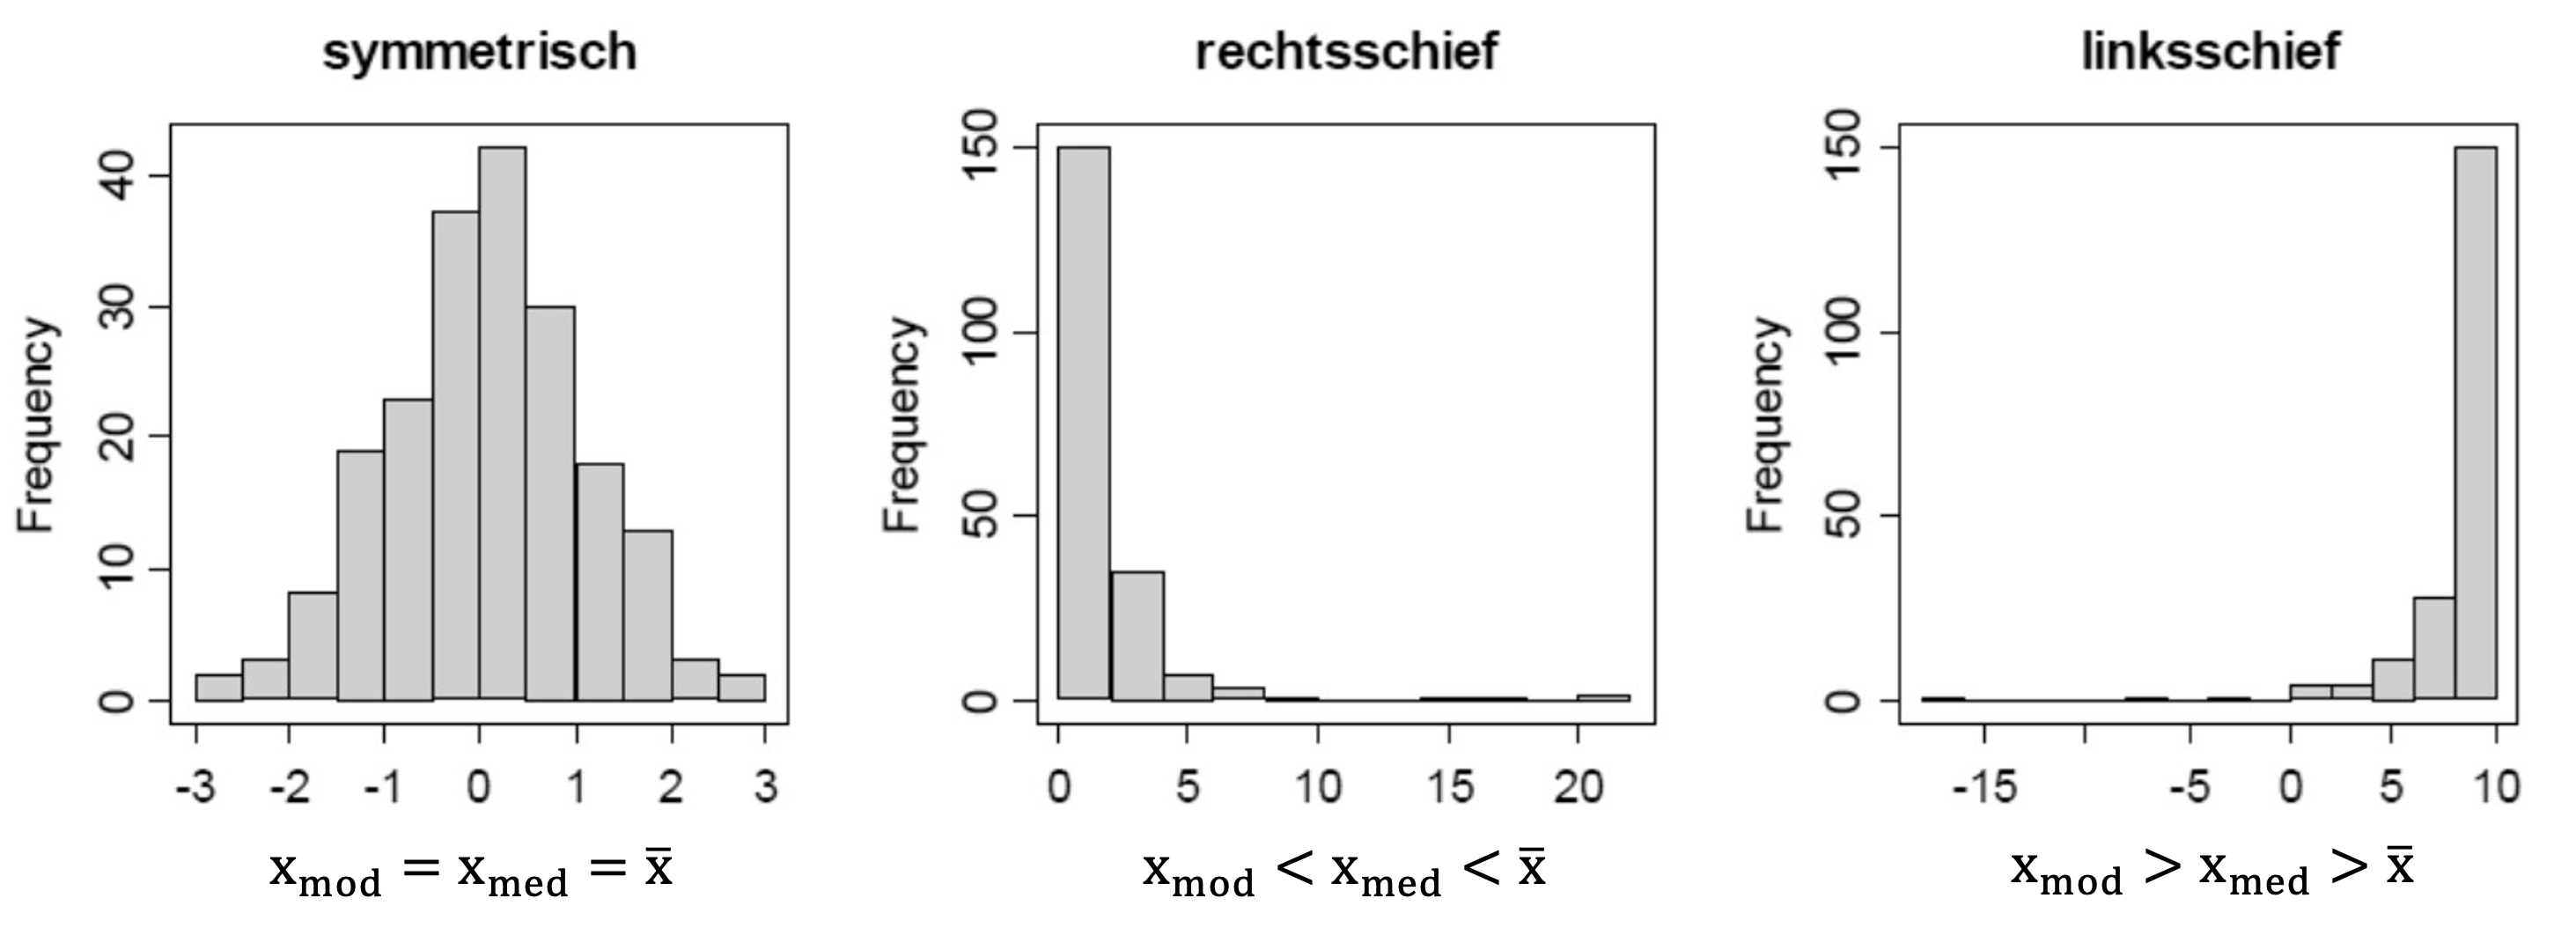
\includegraphics[width=\textwidth]{images/links_rechtsschief.png}
    \end{minipage}
};
\node[fancytitle, right=10pt] at (box.north west) {Form der Verteilung};
\end{tikzpicture}

% Quantile aus Funktion
\begin{tikzpicture}
\node [mybox] (box){
    \begin{minipage}{0.295\textwidth}
	Quantile CMF:\\
	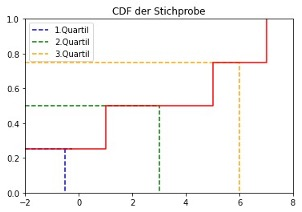
\includegraphics[width=\textwidth]{images/quantile_cmf.jpg}\\
	Quantile CDF:\\
	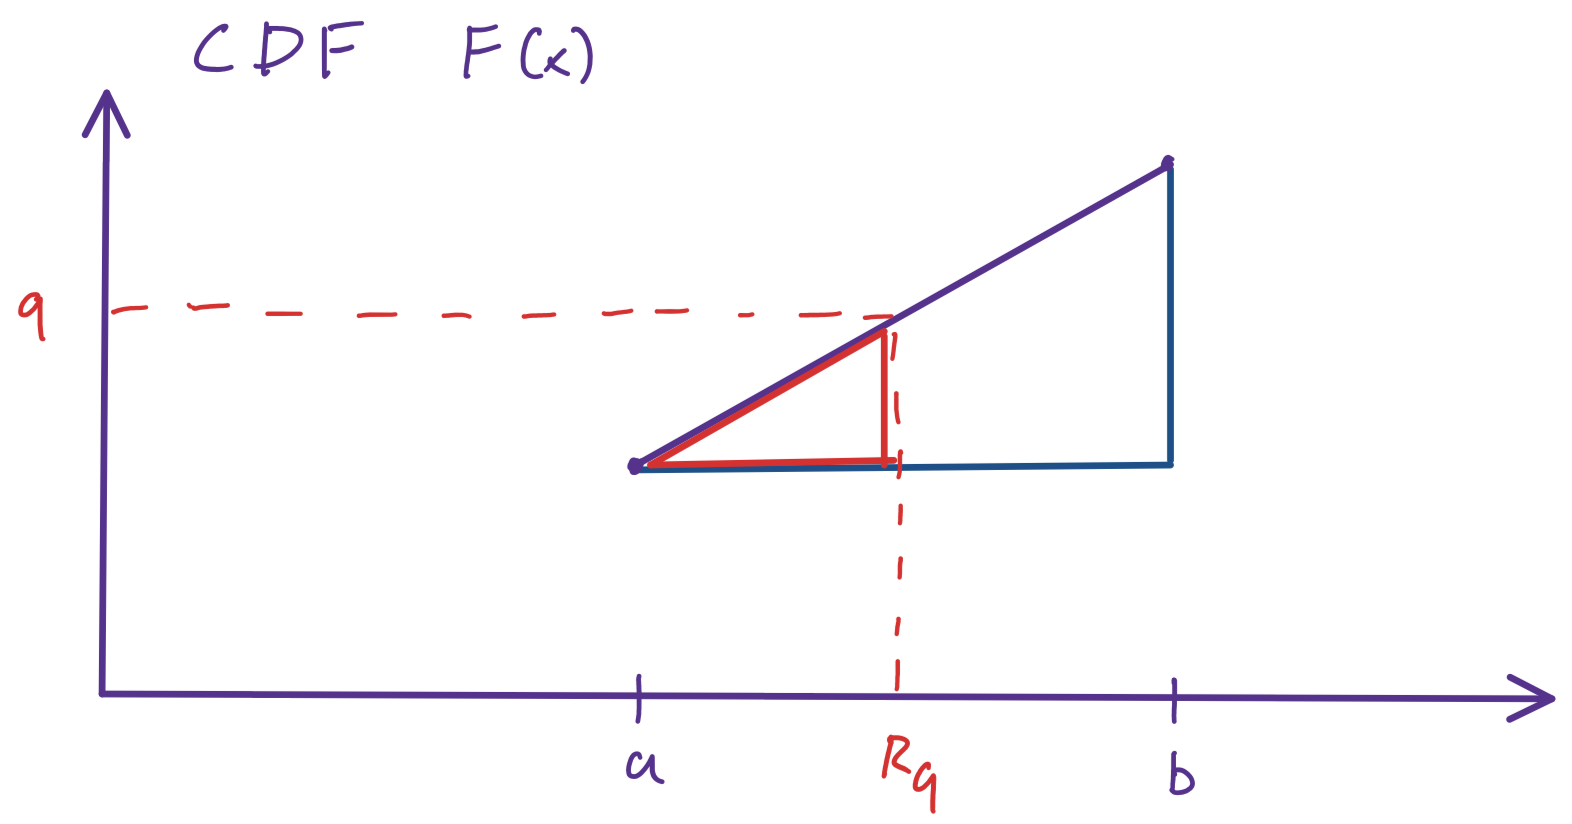
\includegraphics[width=\textwidth]{images/quantile_cdf.png}\\
	Zur Berechnung von $R_q$ sucht man diejenige Klasse $[a,b[$ mit $F(a) \leq q \leq F(b)$
	b
	\begin{itemize}
    \setlength\itemsep{0em}
        \item $m = \frac{q - F(a)}{R_q - a}$
        \item $R_q = a + (b - a)\cdot\frac{q - F(a)}{F(b) - F(a)}$
        \item $q = F(a) + \frac{F(b) - F(a)}{b - a}\cdot(R_q - a)$
        \item $q = F(a) +  f(R_q)\cdot(R_q - a)$
    \end{itemize}
    \end{minipage}
};
\node[fancytitle, right=10pt] at (box.north west) {Quantile aus Funktion};
\end{tikzpicture}


% boxplot
\begin{tikzpicture}
\node [mybox] (box){
    \begin{minipage}{0.295\textwidth}
    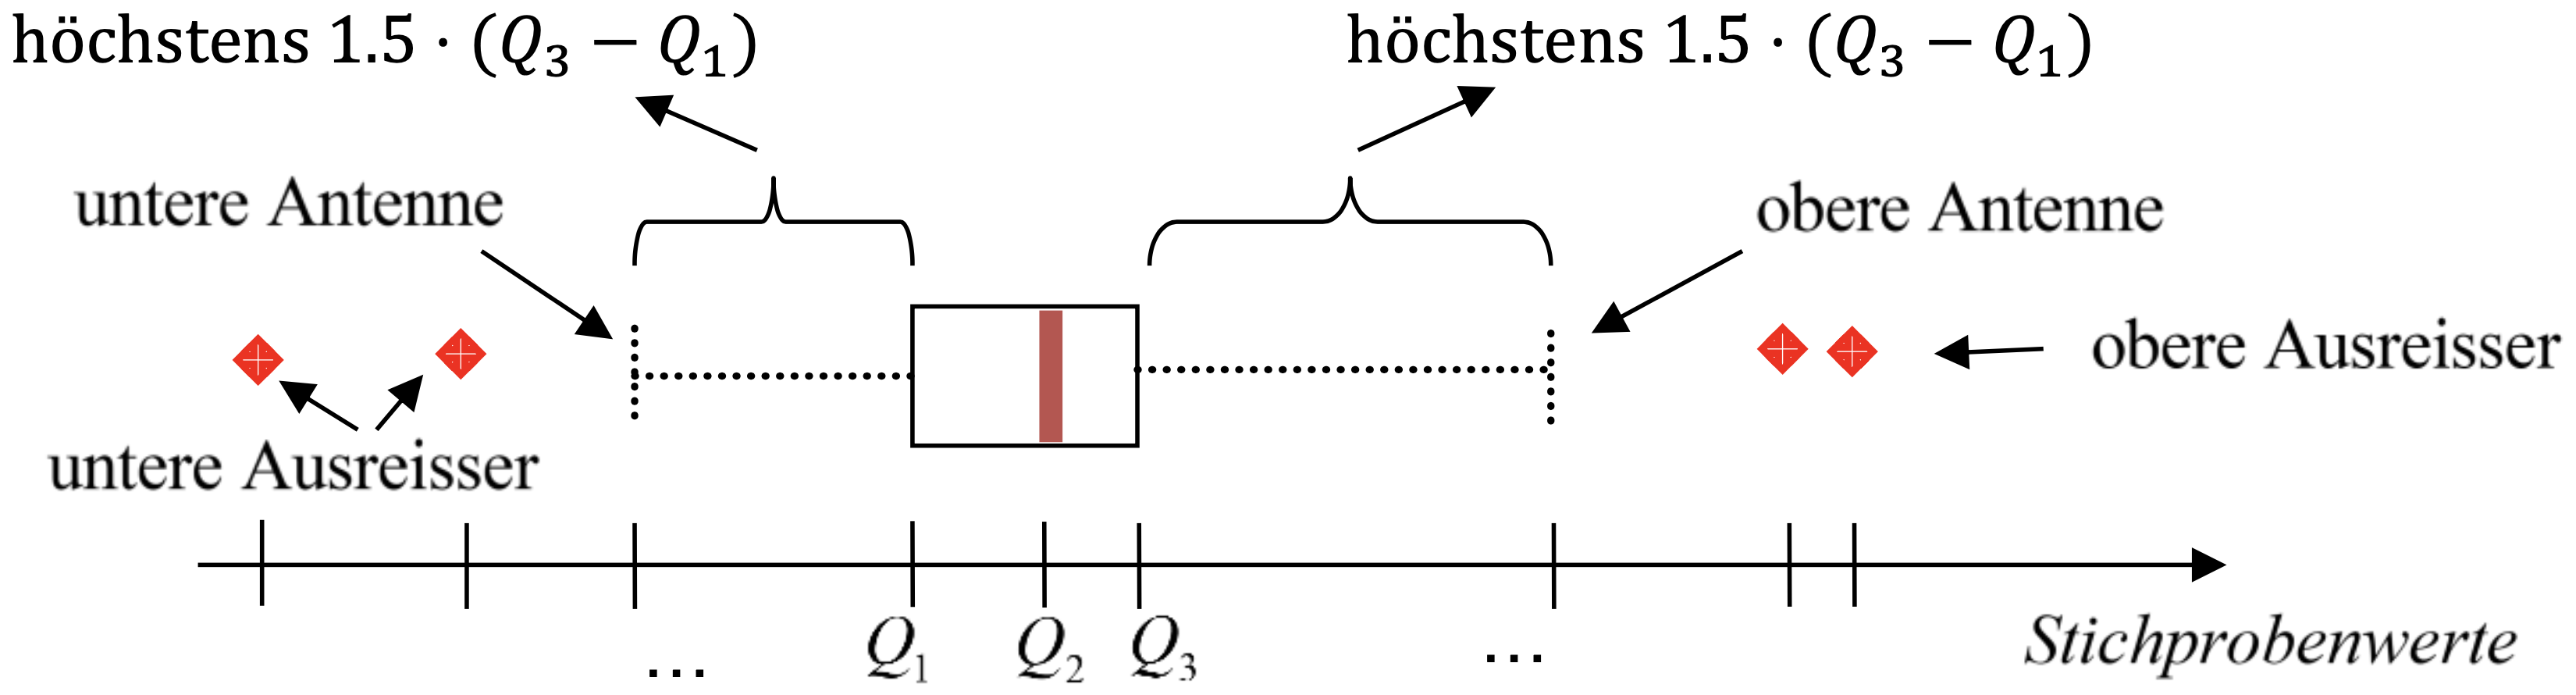
\includegraphics[width=\textwidth]{images/boxplot.png}\\
    Untere und obere Antenne sind Stichprobenwerte!
    \end{minipage}
};
\node[fancytitle, right=10pt] at (box.north west) {Boxplot};
\end{tikzpicture}


\begin{tikzpicture}
\node [mybox] (box){
    \begin{minipage}{0.295\textwidth}
    \begin{tabular}{lp{6.5cm} l}
        $n$: & Anzahl Stichprobenelemente\\
        $m$: & Anzahl Merkmahle\\
        $a_i$: & Stichprobenwert\\
	\end{tabular}
    \begin{itemize}
    \setlength\itemsep{0em}
        \item $\overline{x} = \frac{1}{n}\sum\limits_{i=1}^{n} x_i = \frac{1}{n}\sum\limits_{i=0}^{m} a_i 
        \cdot h_i = \sum\limits_{i=1}^{m} a_i \cdot f_i$
        \item $s_x^2 = \frac{1}{n}\sum\limits_{i=1}^{n} {(x_i - \overline{x})}^2 =
        [\sum\limits_{i=1}^{m} a_i^2 \cdot f_i] - \overline{x}^2$
        \item $s_x = \sqrt{s_x^2}$
        \item $s_{kor}^2 = \frac{1}{n-1}\sum\limits_{i=1}^{n} {(x_i - \overline{x})}^2 =
        \frac{n}{n-1}\cdot s_x^2$
        \item $s_{kor} = \sqrt{s_{kor}^2} = \sqrt{\frac{n}{n-1}}\cdot s_x$
    \end{itemize}
    \end{minipage}
};
\node[fancytitle, right=10pt] at (box.north west) {Lage- und Streumasse};
\end{tikzpicture}


\begin{tikzpicture}
\node [mybox] (box){
    \begin{minipage}{0.295\textwidth}
    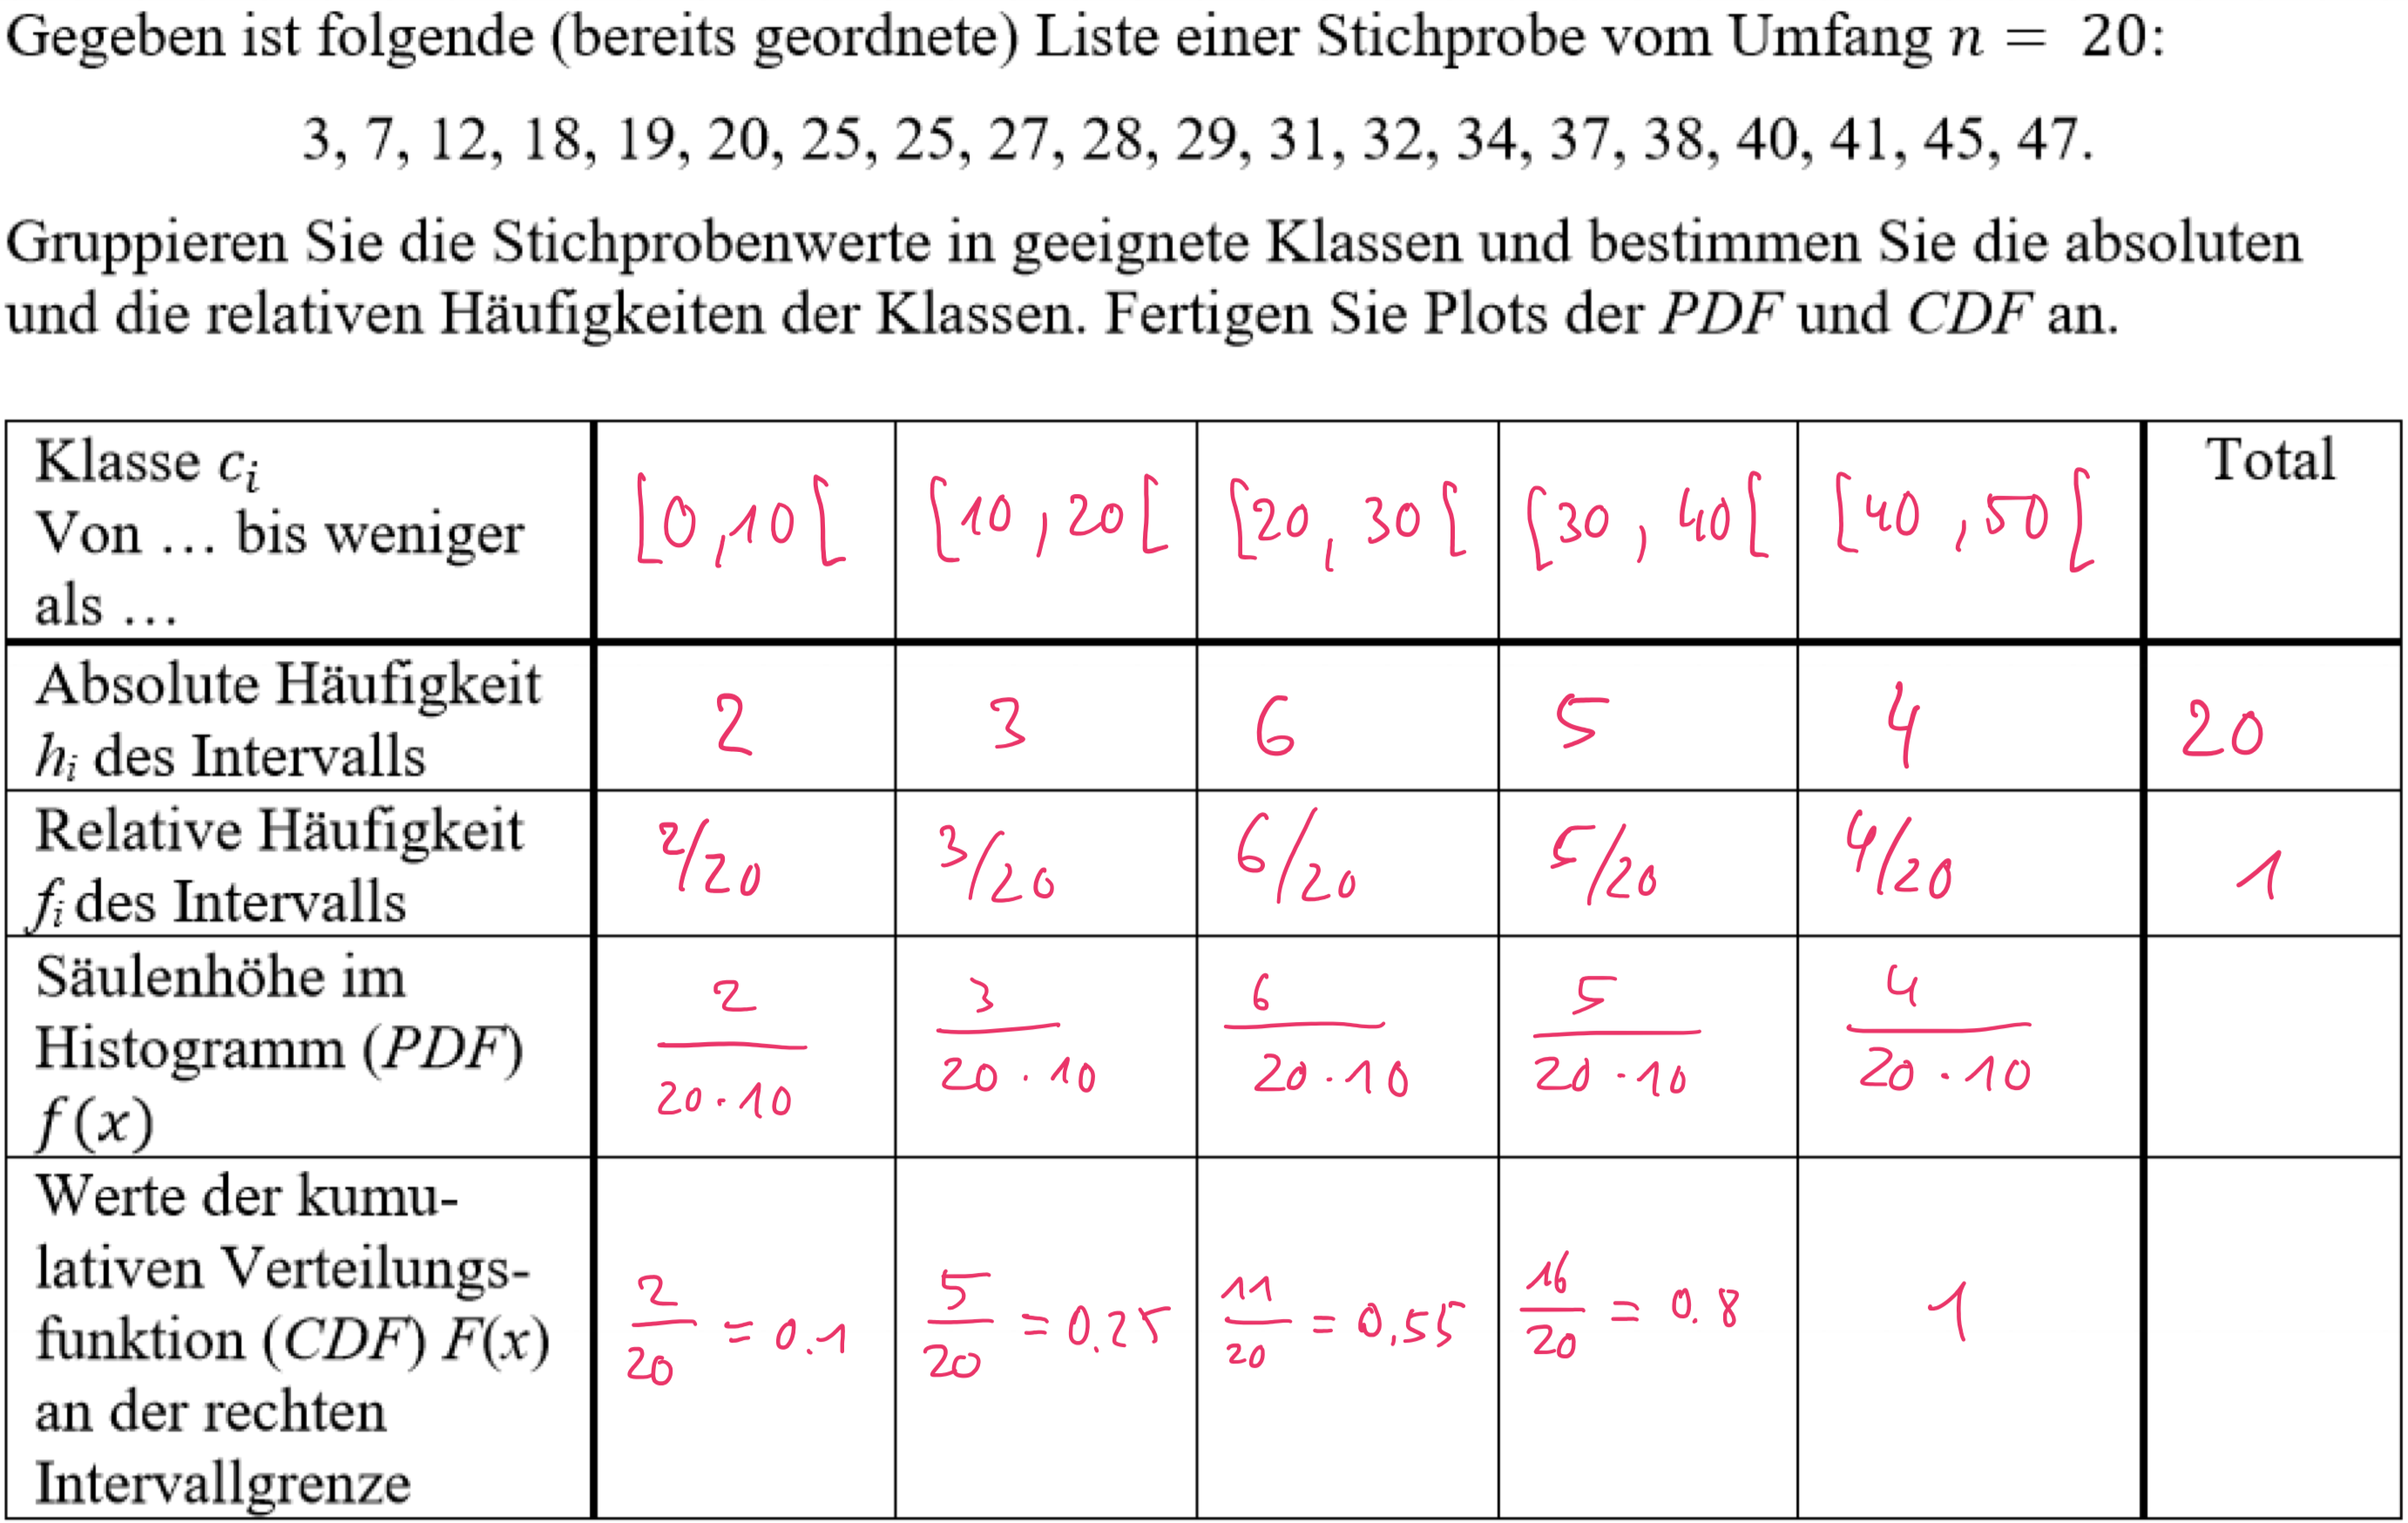
\includegraphics[width=\textwidth]{images/bsp_histogramm.png}
    \end{minipage}
};
\node[fancytitle, right=10pt] at (box.north west) {Bsp. klassierte Stichprobe};
\end{tikzpicture}
\end{multicols}
\newpage








% --------------------------------------------------------------------
% deskriptive Statistik mit mehrere Merkmale
% --------------------------------------------------------------------
\section*{Deskriptive Statistik mit mehrere Merkmale}
\begin{multicols}{3}

% grundbegriffe
\begin{tikzpicture}
\node [mybox] (box){
    \begin{minipage}{0.295\textwidth}
    \begin{tabular}{lp{6.5cm} l}
        $s_{xy}$: & Kovarianz\\
        $r_{xy}$: & Korrelationskoeffizient oder normierte Kovarianz (Pearson)\\
        $r_{sp}$: & Korrelationskoeffizient nach Spearman oder Rangkorrelationskoeffizient\\
        $s_x$: & Standardabweichung der $x_i$ Werte\\
        $s_y$: & Standardabweichung der $y_i$ Werte\\
        $\overline{x}$: & Arithmetisches Mittel der $x_i$\\
        $\overline{y}$: & Arithmetisches Mittel der $y_i$
	\end{tabular}
    \end{minipage}
};
\node[fancytitle, right=10pt] at (box.north west) {Grundbegriffe};
\end{tikzpicture}


% Mittelwerte
\begin{tikzpicture}
\node [mybox] (box){
    \begin{minipage}{0.295\textwidth}
    \begin{multicols}{2}
    \begin{itemize}
    \setlength\itemsep{0em}
        \item $\overline{x} =\frac{1}{n}\sum\limits_{i=1}^{n} x_i$
        \item $\overline{y} =\frac{1}{n}\sum\limits_{i=1}^{n} y_i$
    \end{itemize}
    \begin{itemize}
    \setlength\itemsep{0em}
        \item $\overline{xy} =\frac{1}{n}\sum\limits_{i=1}^{n} x_i y_i$
        \item $\overline{x^2} =\frac{1}{n}\sum\limits_{i=1}^{n} x_i^2$
        \item $\overline{y^2} =\frac{1}{n}\sum\limits_{i=1}^{n} y_i^2$
    \end{itemize}
    \end{multicols}
    \end{minipage}
};
\node[fancytitle, right=10pt] at (box.north west) {Mittelwerte};
\end{tikzpicture}


% Korrelation Pearson
\begin{tikzpicture}
\node [mybox] (box){
    \begin{minipage}{0.295\textwidth}
    \begin{itemize}
    \setlength\itemsep{0em}
        \item $s_x^2 = \overline{x^2} - \overline{x}^2$
        \item $s_x = \sqrt{s_x^2}$
        \item $s_x^2 = \overline{x^2} - \overline{x}^2$
        \item $s_x = \sqrt{s_x^2}$
        \item $s_{xy} = \frac{1}{n}\sum\limits_{i=1}^{n} (x_i - \overline{x})(y_i - \overline{y})$
        \item $s_{xykor} = \frac{1}{n-1}\sum\limits_{i=1}^{n} (x_i - \overline{x})(y_i - \overline{y})$
        \item $r_{xy} = \frac{s_{xy}}{s_x \cdot s_y} = \frac{s_{xykor}}{s_{xkor} \cdot s_{ykor}}$
    \end{itemize}
    $r_{xy}$ ist im Bereich $[0,1]$. desto näher an $1$, desto grösser ist die Korrelation
    \end{minipage}
};
\node[fancytitle, right=10pt] at (box.north west) {Korrelation (Pearson)};
\end{tikzpicture}


% Korrelation Bsp
\begin{tikzpicture}
\node [mybox] (box){
    \begin{minipage}{0.295\textwidth}
    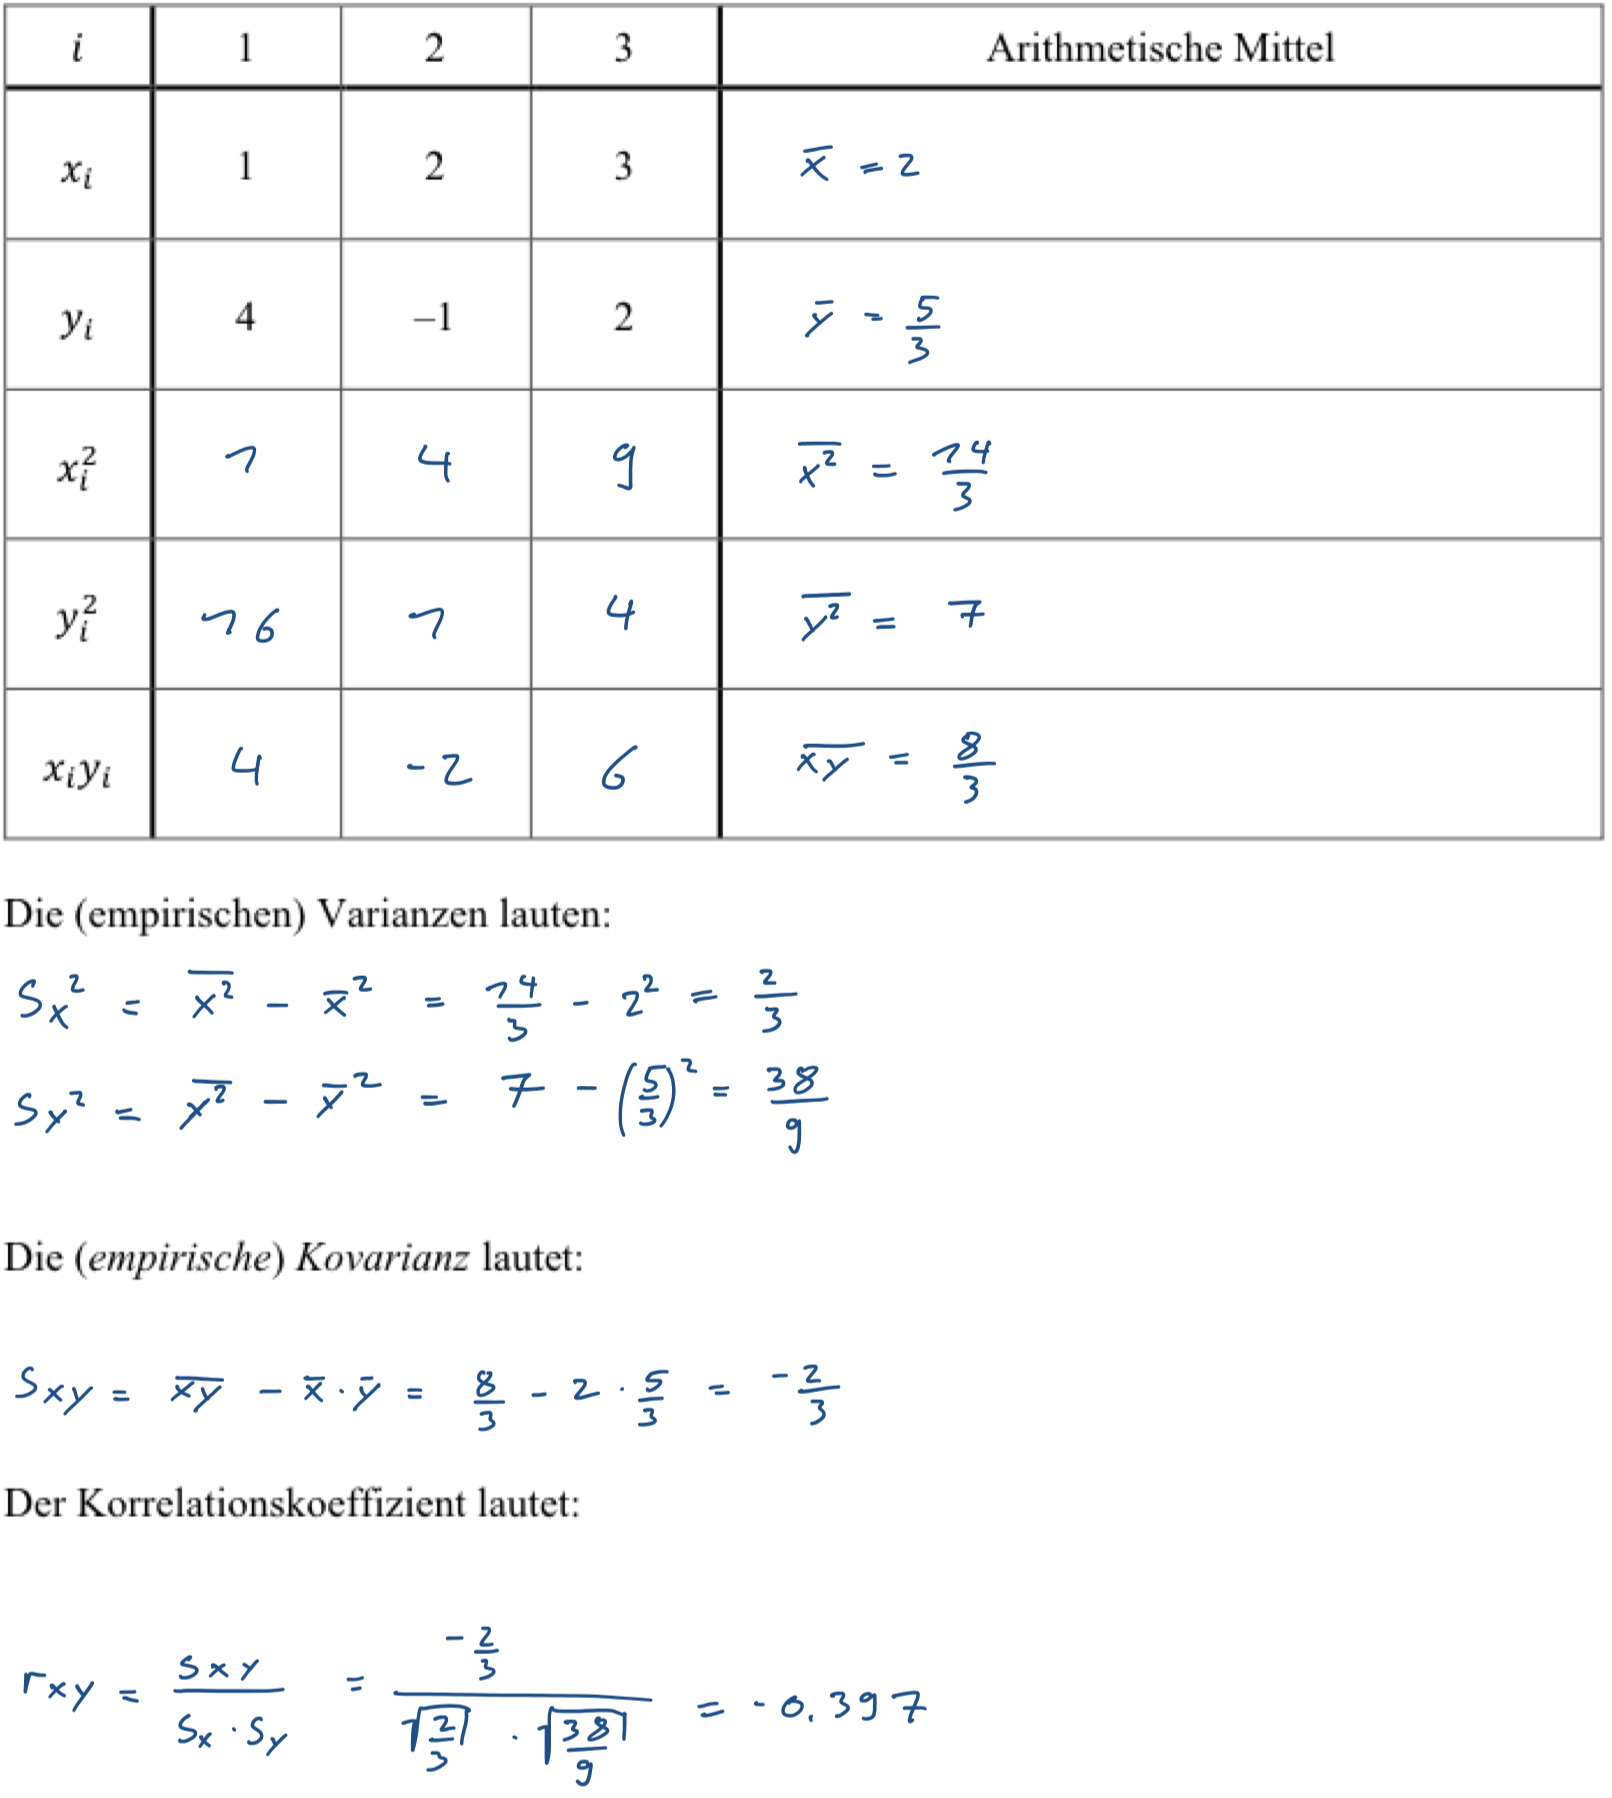
\includegraphics[width=\textwidth]{images/bsp_korrelation.png}
    \end{minipage}
};
\node[fancytitle, right=10pt] at (box.north west) {Bsp. Korrelation};
\end{tikzpicture}


% Korrelation Spearman
\begin{tikzpicture}
\node [mybox] (box){
    \begin{minipage}{0.295\textwidth}
    Bei dem Rankkorrelationskoeffizient werden die Ränge der Stichprobenwerte verwendet.
    um den Rang zu bestimmen können die Werte der Grösse nach sortiert werden.
    \begin{itemize}
    \setlength\itemsep{0em}
        \item $r_{sp} = \sum\limits_{i=1}^{n} {(rg(x_i)-\overline{rg(x_i})}^2$
    \end{itemize}
    Falls der gleiche Stichprobenwert mehrmals vorkommt muss der Rang addiert und durch die Anzahl Vorkomtnisse subtrahiert werden.\\
    Bsp. Verbundene Ränge:\\
    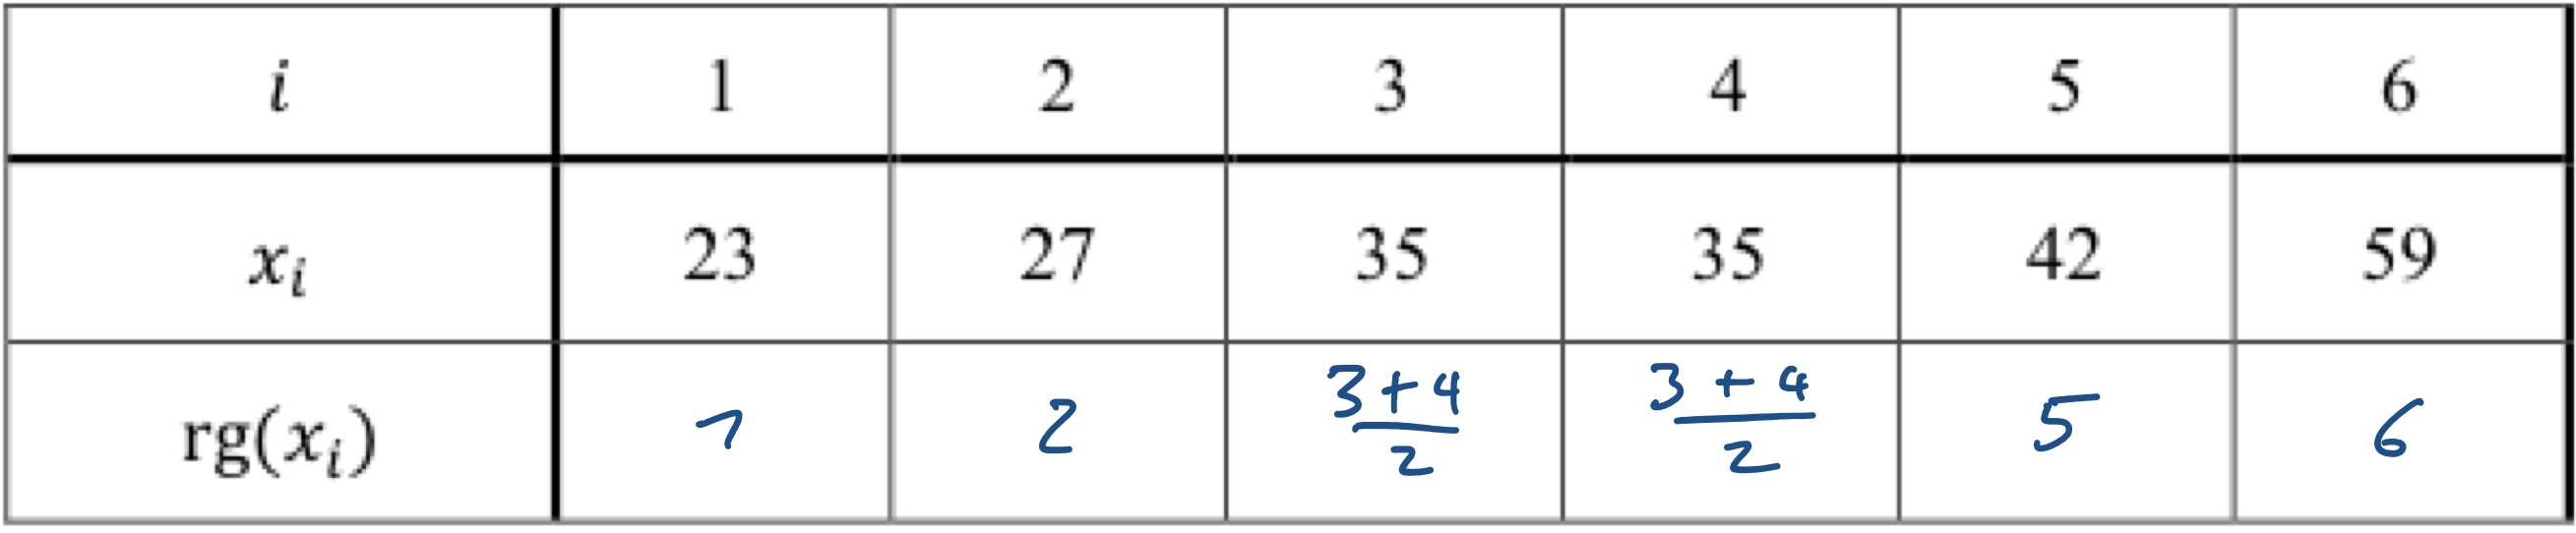
\includegraphics[width=\textwidth]{images/verbundene_raenge.png}
    \end{minipage}
};
\node[fancytitle, right=10pt] at (box.north west) {Korrelation (Spearman)};
\end{tikzpicture}
\end{multicols}
\newpage





% --------------------------------------------------------------------
% Kombinatorik
% --------------------------------------------------------------------
\section*{Kombinatorik}
\begin{multicols}{3}


% Problem
\begin{tikzpicture}
\node [mybox] (box){
    \begin{minipage}{0.295\textwidth}
    \begin{itemize}
    \setlength\itemsep{0em}
        \item \textbf{Zahlenschlossproblem}: Sie haben den Zahlencode ihres Zahlenschlosses vergessen. Das Schloss besteht aus 6 Zahlenkränzen mit den Zahlen 0 bis 9. Wie viele Einstellungen müssen Sie im schlimmsten Fall probieren, um ihren Zahlencode zu finden?
        \item \textbf{Schwimmwettkampf}: Bei einem Schwimmwettbewerb starten 10 Schwimmerinnen. Wie viele mögliche Platzierungen gibt es, wenn Sie nur die ersten drei Plätze betrachten und nicht zulassen, dass Schwimmerinnen zeitgleich im Ziel ankommen können?
        \item \textbf{Lotto}: Wie gross sind die Chancen beim Lotto 6 aus 49 mit einem Versuch sechs richtige Zahlen vorauszusagen?
        \item \textbf{Bitproblem}: Wie viele verschiedene natürliche Zahlen können mit 64 Bits binär dargestellt werden?
        \item \textbf{Zahnarztproblem}: Eine Zahnärztin erlaubt den Kindern, nach der Behandlung zur Belohnung 3 Spielzeuge aus 5 Töpfen auszusuchen. Die 5 Töpfe sind dabei jeweis mit einer Art Spielzeug befüllt (Gummiball, Spielfigur, Toyauto, Jojo, Kreisel). Wie viele verschiedene Möglichkeiten hat ein Kind?
        \item \textbf{Fussballmannschaft}: Aus einer Klasse mit 20 Studierenden soll eine Fussballmannschaft mit 11 Spielern zusammengestellt werden. (6a) Wie viele Möglichkeiten gibt es? (6b) Wie viele Möglichkeiten gibt es, wenn die Mannschaft genau aus 6 Frauen und 5 Männern bestehen soll und die Klasse aus 8 Frauen und 12 Männern besteht.
    \end{itemize}
    \end{minipage}
};
\node[fancytitle, right=10pt] at (box.north west) {Probleme};
\end{tikzpicture}


% Problem
\begin{tikzpicture}
\node [mybox] (box){
    \begin{minipage}{0.295\textwidth}
    \begin{itemize}
    \setlength\itemsep{0em}
        \item \textbf{Buchstabenproblem}: Mit 10 verschiedenen Buchstaben sollen Wörter von 5 Zeichen gebildet werden. (7a) Wie viele solche Wörter gibt es, wenn dabei kein Buchstabe doppelt vorkommen darf. (7b) Wie viele verschiedene Wörter gibt es, wenn Buchstaben mehrmals vorkommen können.
        \item \textbf{Tellschiessen}: Wilhelm Tell schiesst mit drei Pfeilen auf eine Zielscheibe, welche in 10 ringförmige Bereiche unterteilt ist. Wie viele verschiedene Resultate gibt es für Wilhelm?
        \item \textbf{Napoleon}: schart seine 10 Generäle für eine Beratung um sich an einem kreisrunden Tisch mit 11 Plätzen. (9a) Wie viele verschiedene Sitzreihenfolgen gibt es? (9b) Wie viele verschiedene Sitzreihenfolgen gibt es, wenn Napoleons Liebling Marschall Ney immer an Napoleons Seite sitzen soll?
        \item \textbf{Gruppen}: Wie viele verschiedene Personengruppen kann man aus einer Klasse mit 20 Studierenden bilden?
        \item \textbf{Teilmengen}: (11a) Wie viele dreielementige Teilmengen hat die Menge {1,2,3,4}? (11b) Wie viele Teilmengen hat die Menge {1,2,3,4}? Wie viele Teilmengen hat eine Menge mit n Elementen?
    \end{itemize}
    \end{minipage}
};
\node[fancytitle, right=10pt] at (box.north west) {Probleme};
\end{tikzpicture}


% Binominalkoeffizient
\begin{tikzpicture}
\node [mybox] (box){
    \begin{minipage}{0.295\textwidth}
    \textbf{Definition:}
        \begin{itemize}
    \setlength\itemsep{0em}
        \item $\left(\begin{array}{c} n \\ k \end{array}\right) = \frac{n!}{(n-k)! \cdot k!}$
    \end{itemize}
    \textbf{Eigenschaften:}\\
        \begin{tabular}{lp{6.5cm} l}
            Leere Menge: & $\left(\begin{array}{c} n \\ 0 \end{array}\right) = 1$\\\\
            Symmetrie: & $\left(\begin{array}{c} n \\ k \end{array}\right) 
            = \left(\begin{array}{c} n \\ n-k \end{array}\right)$\\\\
            Rekursion: & $\left(\begin{array}{c} n+1 \\ k+1 \end{array}\right)
            = \left(\begin{array}{c} n \\ k \end{array}\right) +
            \left(\begin{array}{c} n \\ k+1 \end{array}\right)$\\\\
            Summe: & $\sum\limits_{k=0}^{n} \left(\begin{array}{c} n \\ k \end{array}\right)
            = 2^n$
	    \end{tabular}
    \end{minipage}
};
\node[fancytitle, right=10pt] at (box.north west) {Binominalkoeffizient};
\end{tikzpicture}


% Abzählprobleme
\begin{tikzpicture}
\node [mybox] (box){
    \begin{minipage}{0.295\textwidth}
    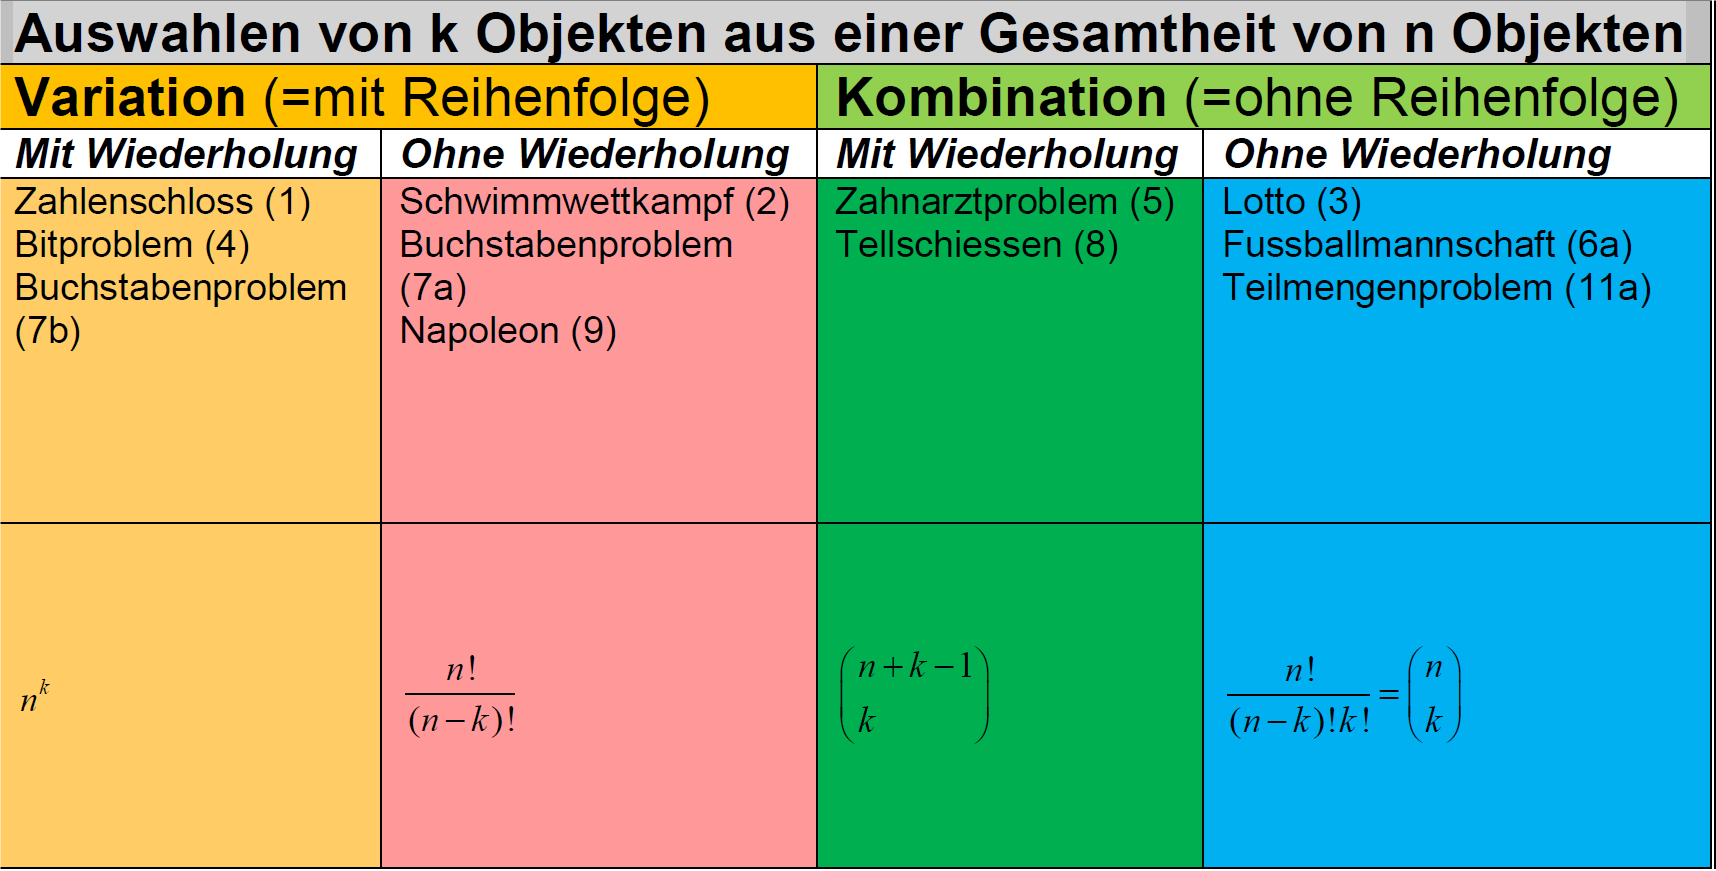
\includegraphics[width=\textwidth]{images/Diagramm_kombinatorik.png}
    \end{minipage}
};
\node[fancytitle, right=10pt] at (box.north west) {Abzählprobleme};
\end{tikzpicture}
\end{multicols}
\newpage





% --------------------------------------------------------------------
% Kombinatorik
% --------------------------------------------------------------------
\section*{Elementare Wahrscheinlichkeitsrechnung}
\begin{multicols}{3}

% grundbegriffe
\begin{tikzpicture}
\node [mybox] (box){
    \begin{minipage}{0.295\textwidth}
    \begin{tabular}{lp{6.5cm} l}
        $\Omega$: & Ergebnisraum. Alle möglichen ergebnisse eines Zufallsexperiments.\\
        $\rho$: & Zähldichte (PMF). $\rho$ ist eine Funktion die angibt mit welcher Wahrscheinlichkeit die möglichen Ergebnisse des Zufallsexperiments auftreten.
	\end{tabular}
    \end{minipage}
};
\node[fancytitle, right=10pt] at (box.north west) {Grundbegriffe};
\end{tikzpicture}


\begin{tikzpicture}
\node [mybox] (box){
    \begin{minipage}{0.295\textwidth}
        \begin{itemize}
        \setlength\itemsep{0em}
            \item (Unmögliches ergebnis) $P({})=0$
            \item (Sicheres ergebnis) $P(\Omega)=1$
            \item (Komplementäres Ereignis) $P(\Omega \setminus A)= 1 - P(A)$
            \item (Vereinigung) $P(A \cup B) = P(A) + P(B) - P(A \cap B)$
            \item (Sigma-Additivität) \\$P(A_1 \cup A_2 \cup A_3 \cup \ldots) = P(A_1)
            + P(A_2) + P(A_3) + \ldots$
            \item Ist $(\Omega , P)$ ein Laplace-Raum, so gilt: $P(M)= \frac{|M|}{|\Omega|}$
        \end{itemize}
    \end{minipage}
};
\node[fancytitle, right=10pt] at (box.north west) {Diskreter Wahrscheinlichkeitsraum};
\end{tikzpicture}


\begin{tikzpicture}
\node [mybox] (box){
    \begin{minipage}{0.295\textwidth}
        \begin{itemize}
        \setlength\itemsep{0em}
            \item \textbf{Linearität des Erwartungswertes:}\\
            $E(X+Y) = E(X)+E(Y)$ und $E(\alpha X) = \alpha E(X)$
            \item \textbf{Verschiebungssatz für die Varianz:}\\
            $V(X) = E(X^2) - {E(X)^2}$
        \end{itemize}
    \end{minipage}
};
\node[fancytitle, right=10pt] at (box.north west) {Kenngrössen};
\end{tikzpicture}


\begin{tikzpicture}
\node [mybox] (box){
    \begin{minipage}{0.295\textwidth}
        Die Wahrscheinlichkeit für das Eintreten des Ereignisses B, 
        unter Voraussetzung dass das Ereignis A eintritt
        \begin{itemize}
        \setlength\itemsep{0em}
            \item \textbf{Multiplikationssatz} \\
            $P(A \cap B) = P(A) \cdot P(B|A) = P(B) \cdot P(A|B)$
            \item \textbf{Satz von der totalen Wahrscheinlichkeit}\\
            $P(B) = P(A) \cdot P(B|A) + P(\overline{A}) \cdot P(B|\overline{A})$
            \item \textbf{Satz von Bayes}\\
            $P(B|A) = \frac{P(A \cap B)}{P(A)}$
        \end{itemize}
    \end{minipage}
};
\node[fancytitle, right=10pt] at (box.north west) {Bedingte Wahrscheinlichkeit};
\end{tikzpicture}

\begin{tikzpicture}
\node [mybox] (box){
    \begin{minipage}{0.295\textwidth}
        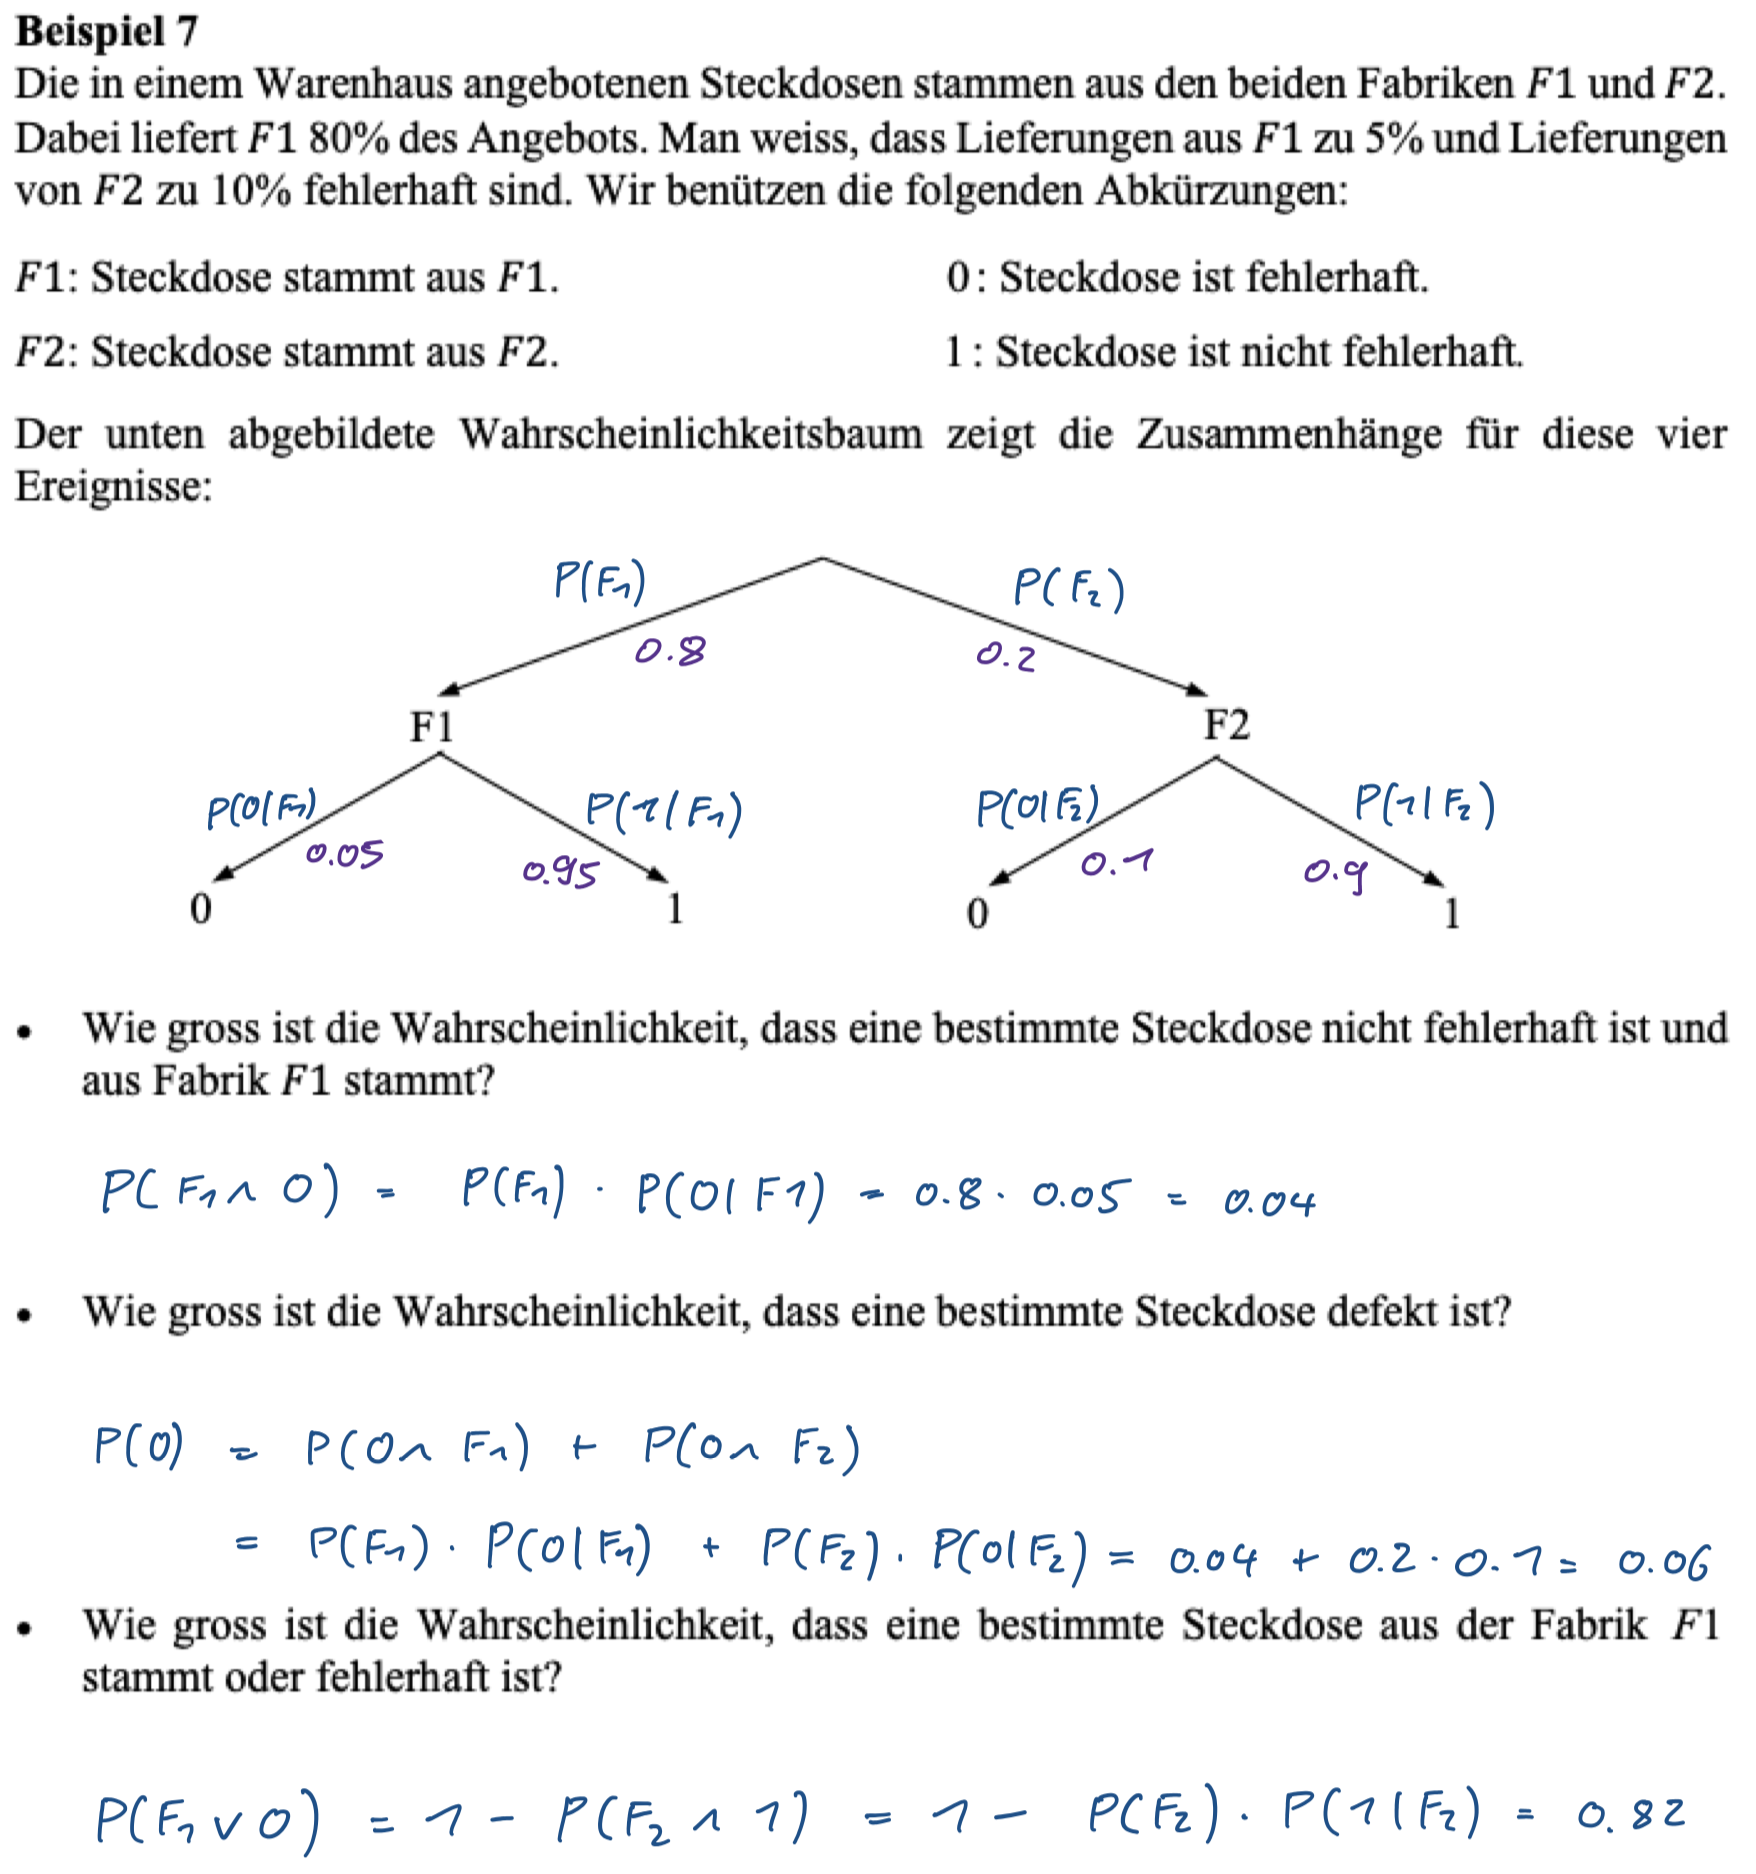
\includegraphics[width=\textwidth]{images/Bsp_Ereignisbaum_1.png}
        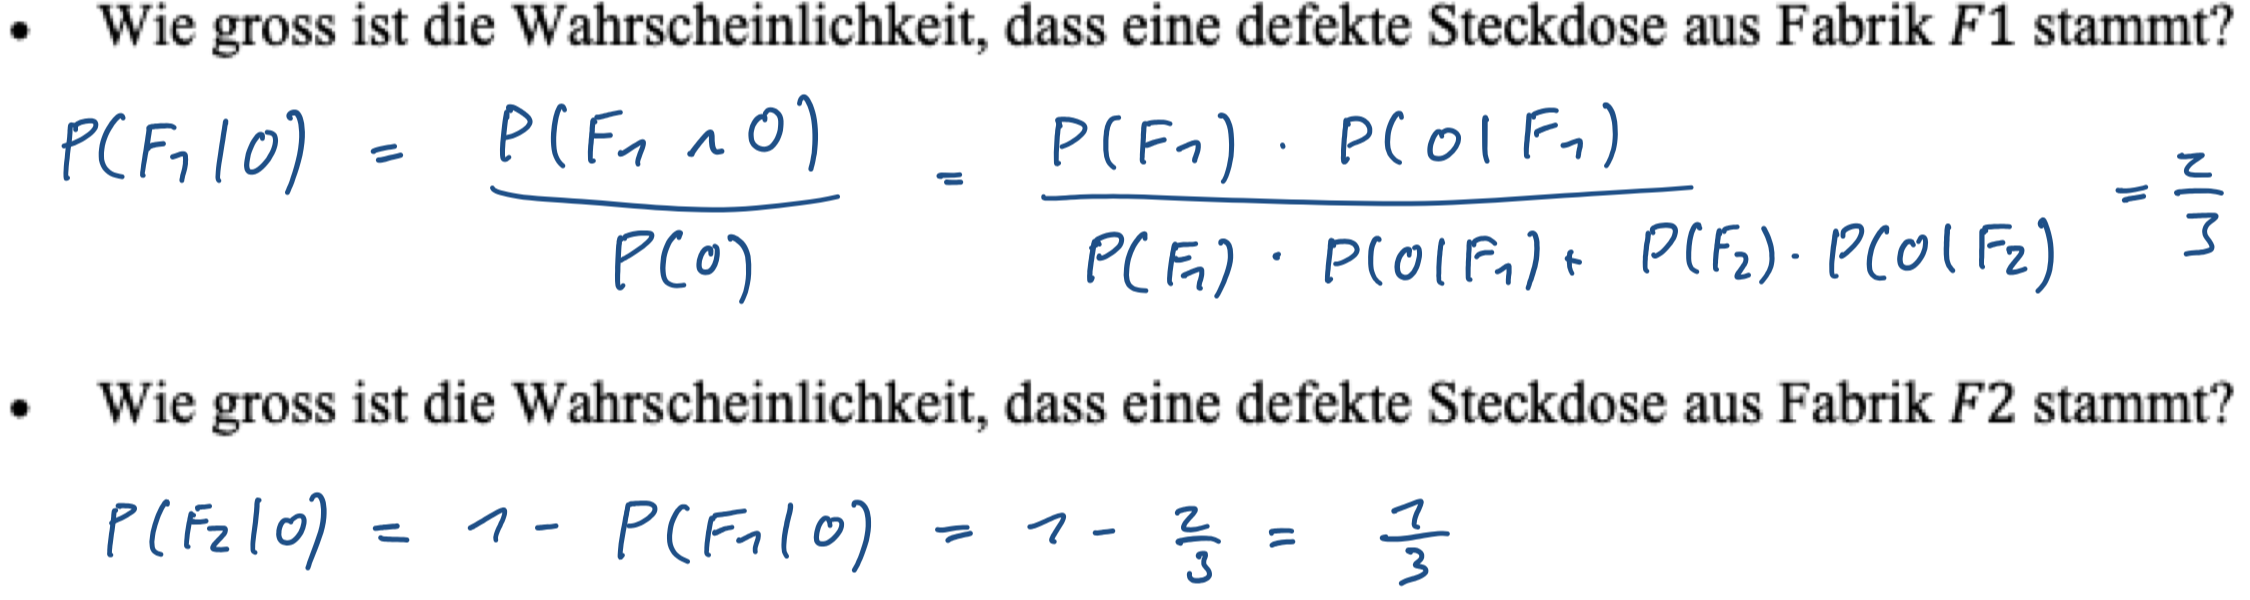
\includegraphics[width=\textwidth]{images/Bsp_Ereignisbaum_2.png}
    \end{minipage}
};
\node[fancytitle, right=10pt] at (box.north west) {Bsp. Ereignisbaum};
\end{tikzpicture}



\begin{tikzpicture}
\node [mybox] (box){
    \begin{minipage}{0.295\textwidth}
        Falls zwei Ereignisse stochastisch unabhängig sind, beeinflusst das
        Eintreten des einen Ereignisses nicht das Eintreten des Anderen. somit gilt:
        \begin{itemize}
        \setlength\itemsep{0em}
            \item $P(A|B) = P(A)$ und $P(B|A) = P(B)$
        \end{itemize}
        Für zwei Ereignisses $A$ und $B$ sind folgende Aussagen equivalent:
        \begin{itemize}
        \setlength\itemsep{0em}
            \item $A$ und $B$ sind stochastisch unabhängig
            \item $A$ und $\Omega \setminus B$ sind stochastisch unabhängig
            \item $\Omega \setminus A$ und $\Omega \setminus B$ sind stochastisch unabhängig
        \end{itemize}
        Für stochastisch unabhängige Zufallsvariablen $X$,$Y$ gilt:
        \begin{itemize}
        \setlength\itemsep{0em}
            \item $E(X \cdot Y) = E(X) \cdot E(Y)$
            \item $V(X + Y) = V(X) + V(Y)$
        \end{itemize}
    \end{minipage}
};
\node[fancytitle, right=10pt] at (box.north west) {Stochastische Unabhängigkeit};
\end{tikzpicture}


\begin{tikzpicture}
\node [mybox] (box){
    \begin{minipage}{0.295\textwidth}
        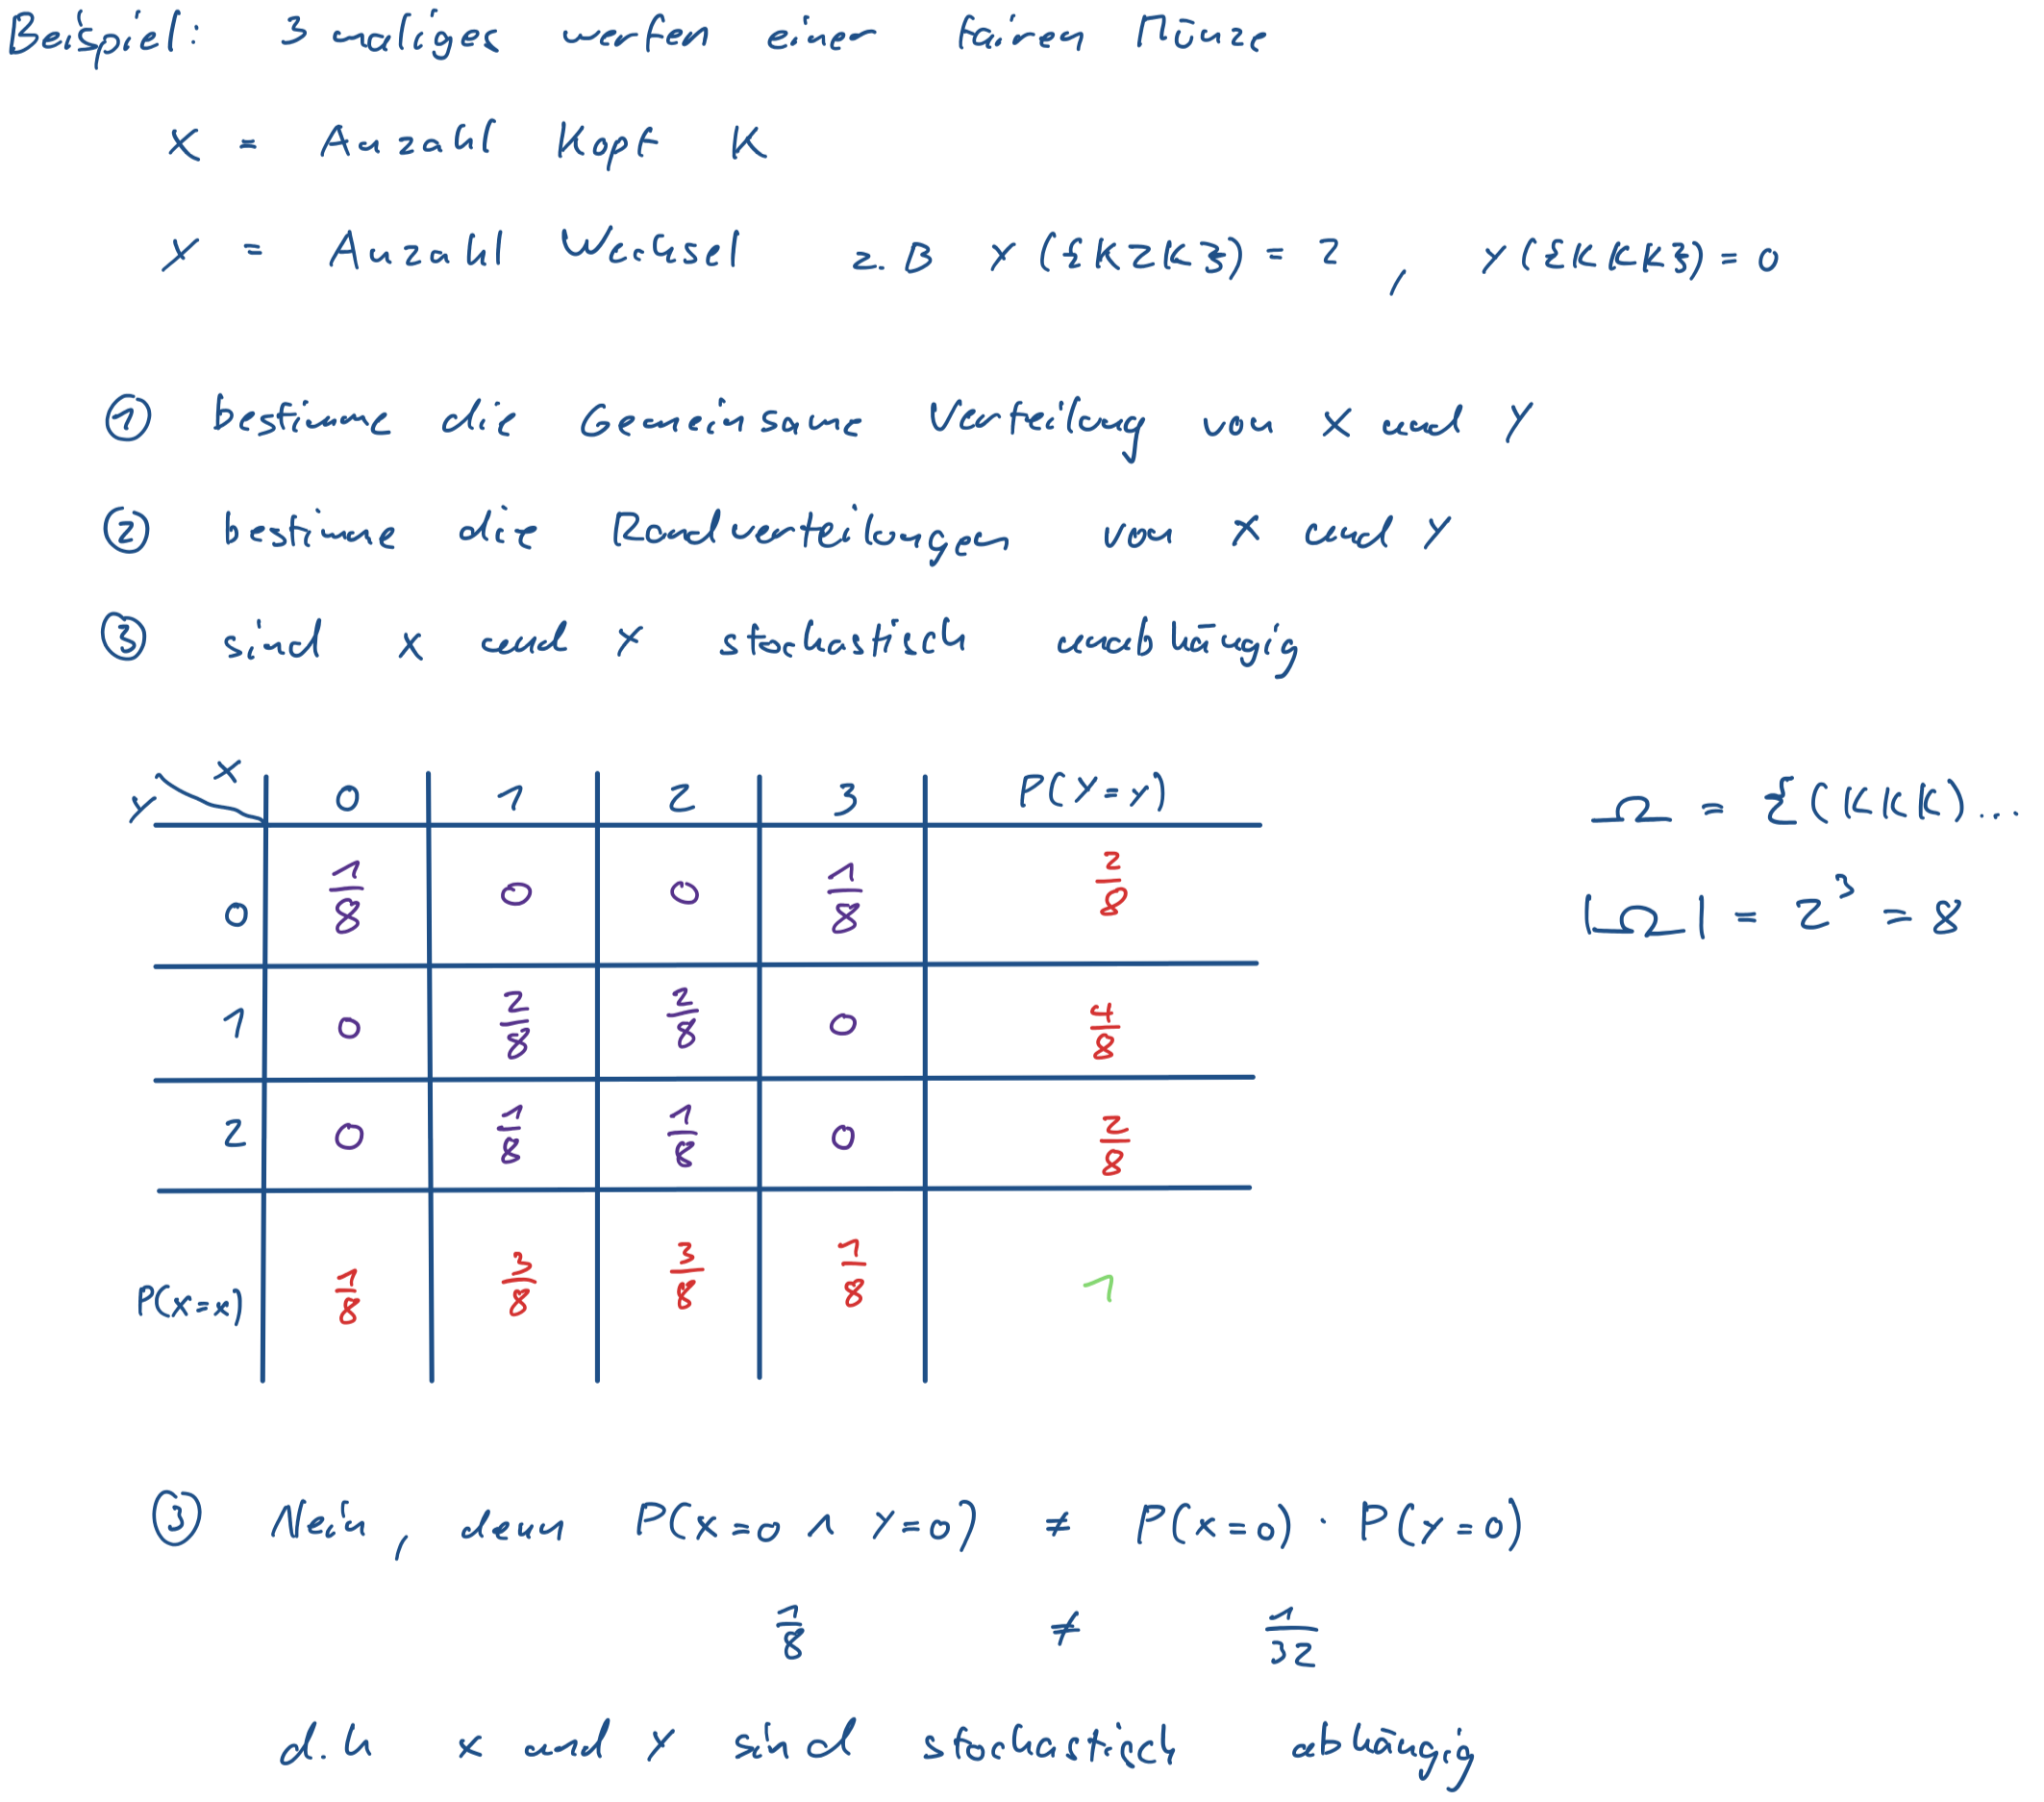
\includegraphics[width=\textwidth]{images/bsp_stoch_abhaengigkeit.png}
    \end{minipage}
};
\node[fancytitle, right=10pt] at (box.north west) {Bsp. Stochastische Unabhängigkeit};
\end{tikzpicture}


\end{multicols}
\newpage





% --------------------------------------------------------------------
% Spezielle Verteilungen
% --------------------------------------------------------------------
\section*{Spezielle Verteilungen}

\begin{multicols}{3}


% grundbegriffe
\begin{tikzpicture}
\node [mybox] (box){
    \begin{minipage}{0.295\textwidth}
    \begin{tabular}{lp{6.5cm} l}
        $\Omega$: & Ergebnisraum. Alle möglichen ergebnisse eines Zufallsexperiments.\\
        $\rho$: & Zähldichte (PMF). $\rho$ ist eine Funktion die angibt mit welcher Wahrscheinlichkeit die möglichen Ergebnisse des Zufallsexperiments auftreten.\\
        $E(X)$: & Erwartungswert\\
        $V(X)$: & Varianz\\
        $S(X)$: & Standardabweichung
	\end{tabular}
    \end{minipage}
};
\node[fancytitle, right=10pt] at (box.north west) {Grundbegriffe};
\end{tikzpicture}


\begin{tikzpicture}
\node [mybox] (box){
    \begin{minipage}{0.295\textwidth}
        \includegraphics[width=\textwidth]{images/diskrete_stetige_Zufallsvariablen.png}
    \end{minipage}
};
\node[fancytitle, right=10pt] at (box.north west) {Diskrete und stetige Zufallsvariablen};
\end{tikzpicture}


\begin{tikzpicture}
\node [mybox] (box){
    \begin{minipage}{0.295\textwidth}
        Eine diskrete Zufallsvariable $X$ heisst hypergeometrisch verteilt mit
        Parametern: $n$ Objekte aus einer Gesamtheit von $N$ Objekten mit $M$
        Merkmalsträgern und $N-M$ andersartigen Objekten, wenn Sie die folgende
        Verteilung besitzt:
        \begin{itemize}
            \setlength\itemsep{0em}
                \item Schreibweise: $X \sim H(N,M,n)$
                \item $P(X = x) = \frac{\left( \begin{array}{c} M \\ x \end{array} \right)
                \cdot \left( \begin{array}{c} N - M \\ n - x \end{array} \right)}{
                \left( \begin{array}{c} N \\ n \end{array} \right)}$
                \item $\mu = E(X) = n \cdot \frac{M}{N}$
                \item $\sigma^2 = V(X) = n \cdot \frac{M}{N} (1 - \frac{M}{N})\frac{N-n}{N-1}$
                \item $\sigma = S(X) = \sqrt{n \cdot \frac{M}{N} (1 - \frac{M}{N})\frac{N-n}{N-1}}$
            \end{itemize}
    \end{minipage}
};
\node[fancytitle, right=10pt] at (box.north west) {Hypergeometrische Verteilungen};
\end{tikzpicture}
    

\begin{tikzpicture}
\node [mybox] (box){
    \begin{minipage}{0.295\textwidth}
        Eine diskrete Zufallsvariable $X$heisst binomialverteilt mit Parametern
        $n$ (Anzahl Wiederholungen), $p$ (Wahrscheinlichkeit für ein Ergebnis 1)
        und $q=1-p$, wenn ihre Verteilung gegeben ist durch:
        \begin{itemize}
            \setlength\itemsep{0em}
                \item Schreibweise: $X \sim B(n,p)$
                \item $P(X = x) = \left(\begin{array}{c} n \\ x\end{array}\right) \cdot p^x \cdot q^{n-x}$
                \item $\mu = E(X) = n \cdot p$
                \item $\sigma^2 = V(X) = n \cdot p \cdot q$
                \item $\sigma = S(X) = \sqrt{n \cdot p \cdot q}$
        \end{itemize}
       Wenn die Bedingung $n \lesssim \frac{N}{20}$ erfüllt ist, kann die hypergeometrische Verteilung mit den Parametern $n,M,N$ durch die Binomialverteilung angenähert werden:
       \begin{itemize}
        \setlength\itemsep{0em}
            \item $H(N,M,n) \approx B(n,\frac{M}{N})$
        \end{itemize}
    \end{minipage}
};
\node[fancytitle, right=10pt] at (box.north west) {Binomialverteilung};
\end{tikzpicture}


\begin{tikzpicture}
\node [mybox] (box){
    \begin{minipage}{0.295\textwidth}
        Eine diskrete Zufallsvariable $X$ heisst poissonverteilt mit dem
        Parametern $\lambda$, wenn ihre
        Verteilung gegeben ist durch:
        \begin{itemize}
            \setlength\itemsep{0em}
                \item Schreibweise: $X \sim Poi(\lambda)$
                \item $P(X = x) = \frac{\lambda^x}{x!} \cdot e^{-\lambda}$
                \item $\mu = E(X) = \lambda$
                \item $\sigma^2 = V(X) = \lambda$
                \item $\sigma = S(X) = \sqrt{\lambda}$
        \end{itemize}
       Wenn die Bedingungen $n \gtrsim 50$ und $p \lesssim 0.1$ erfüllt sind, kann die Binomialverteilung mit den Parametern $n,p$ durch die Poissonverteilung angenähert werden:
       \begin{itemize}
        \setlength\itemsep{0em}
            \item $B(n,p) \approx Poi(n \cdot p)$
        \end{itemize}
    \end{minipage}
};
\node[fancytitle, right=10pt] at (box.north west) {Poissonverteilung};
\end{tikzpicture}


\begin{tikzpicture}
    \node [mybox] (box){
        \begin{minipage}{0.295\textwidth}
            Die stetige Zufallsvariable $X$ folgt der Normalverteilung mit den Parametern $\mu, \sigma \in \mathbb{R}, \sigma > 0$, wenn sie folgende Dichtefunktion hat:
            \begin{itemize}
                \setlength\itemsep{0em}
                    \item Schreibweise: $X \sim N(\mu;\sigma)$
                    \item $E(X) = \mu$
                    \item $V(X) = \sigma$
            \end{itemize}
            Ist $\mu = 0$ und $\sigma = 1$, so spricht man von der
            \textbf{Standardnormalverteilung}.
            \begin{itemize}
                \setlength\itemsep{0em}
                    \item Schreibweise: $X \sim N(0;1)$
            \end{itemize}
            \textbf{Standardisieren:}\\
            liegt eine beliebige Normalverteilung vor, kann diese
            standartiesiert werden. Statt der ursprünglichen Zufallsvariablen
            $X$ betrachtet man die Zufallsvariable:
            \begin{itemize}
                \setlength\itemsep{0em}
                    \item $U = \frac{X - \mu}{\sigma}$
            \end{itemize}
        \end{minipage}
    };
    \node[fancytitle, right=10pt] at (box.north west) {Normalverteilung};
    \end{tikzpicture}


\begin{tikzpicture}
    \node [mybox] (box){
        \begin{minipage}{0.295\textwidth}
            \begin{itemize}
                \setlength\itemsep{0em}
                    \item $P(X \leq -a) = 1 - P(X \leq a)$
                    \item $P(a \leq X \leq b) = P(X \leq b) - P(X \leq a)$
            \end{itemize}
        \end{minipage}
    };
    \node[fancytitle, right=10pt] at (box.north west) {Rechenregeln Normalverteilung};
    \end{tikzpicture}


\begin{tikzpicture}
    \node [mybox] (box){
        \begin{minipage}{0.295\textwidth}
            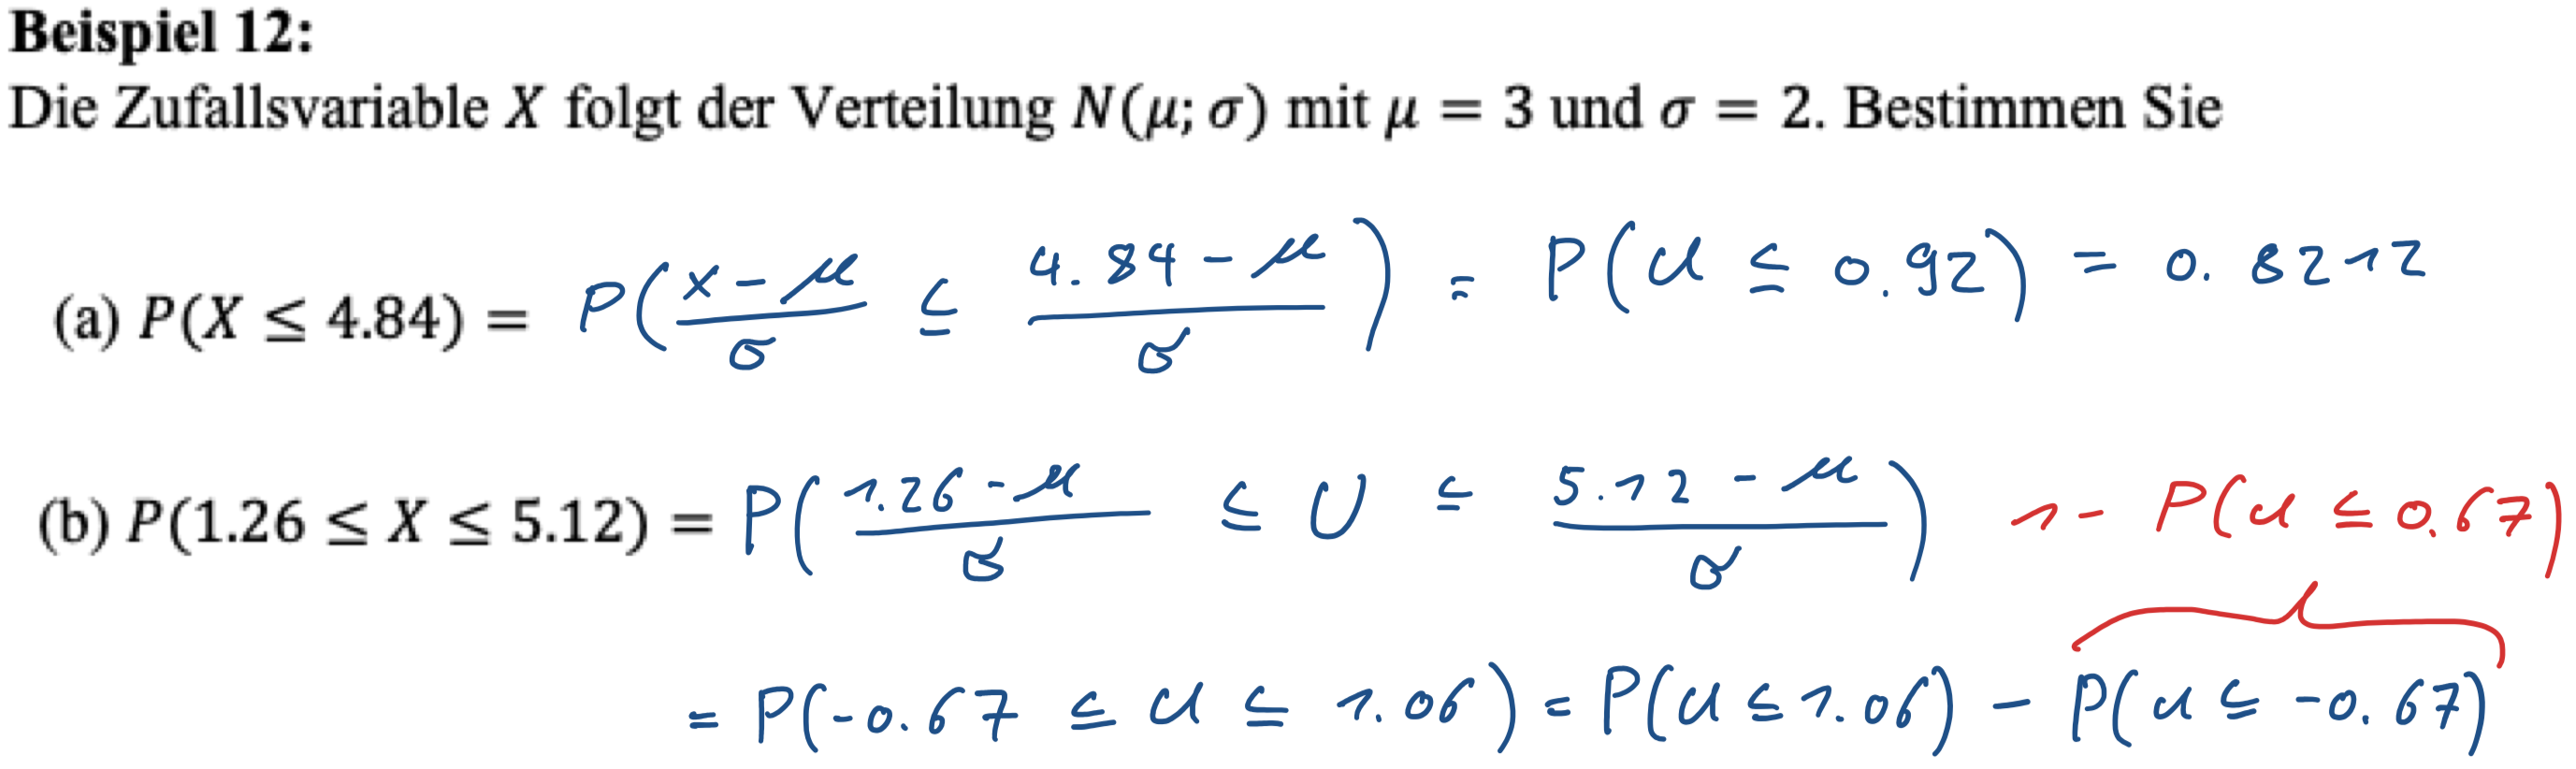
\includegraphics[width=\textwidth]{images/bsp_normalverteilung_standardisieren.png}
        \end{minipage}
    };
    \node[fancytitle, right=10pt] at (box.north west) {Bsp. Standardisieren};
    \end{tikzpicture}


\begin{tikzpicture}
    \node [mybox] (box){
        \begin{minipage}{0.295\textwidth}
            Zufallsvariablen $X_1,\cdots,X_n$ stochastisch unabhängig und
            identisch verteilt $E(X_i)= \mu, V(X_i)=\sigma^2$\\\\
            \textbf{Zufallsvariablen:}\\
            \begin{tabular}{lp{6.5cm} l}
                Summe: & $S_n = X_1+\cdots+X_n$\\
                Arith. Mittel: & $\overline{X_n} = \frac{1}{n} \cdot S_n$\\
	        \end{tabular}\\
            \textbf{$\Rightarrow $}
            \begin{tabular}{lp{6.5cm} l}
                $S_n$ & $\cong_{Approx} N(n \cdot \mu; \sqrt{n} \cdot \sigma)$\\
                $\overline{X_n}$ & $\cong_{Approx} N(\mu; \frac{\sigma}{\sqrt{n}})$\\
	        \end{tabular}
            \begin{multicols*}{2}
                \begin{itemize}
                    \setlength\itemsep{0em}
                        \item $E(S_n) = n \cdot \mu$
                        \item $V(S_n) = n \cdot \sigma^2$
                \end{itemize}
                \begin{itemize}
                    \setlength\itemsep{0em}
                        \item $E(\overline{X_n}) = \mu$
                        \item $V(\overline{X_n}) = \frac{\sigma^2}{n}$
                \end{itemize}
            \end{multicols*}
        \end{minipage}
    };
    \node[fancytitle, right=10pt] at (box.north west) {Zentraler Grenzwertsatz};
    \end{tikzpicture}


\begin{tikzpicture}
    \node [mybox] (box){
        \begin{minipage}{0.295\textwidth}
            \textbf{Binomialverteilung:}\\
            Zufallsvariable $X \sim B(n,p)$ mit $npq > 9:$\\
            \begin{tabular}{lp{6.5cm} l}
                $\mu$ & $= n\cdot p$\\
                $\sigma^2$ & $= n \cdot p \cdot q$\\
	        \end{tabular}\\\\
            \textbf{Poissonverteilung:}\\
            Zufallsvariable $X \sim Poi(\lambda)$ mit $\lambda > 9:$\\
            \begin{tabular}{lp{6.5cm} l}
                $\mu$ & $= \lambda$\\
                $\sigma^2$ & $= \lambda$
	        \end{tabular}
        \end{minipage}
    };
    \node[fancytitle, right=10pt] at (box.north west) {Approximationen durch Normalverteilung};
    \end{tikzpicture}


\begin{tikzpicture}
    \node [mybox] (box){
        \begin{minipage}{0.295\textwidth}
            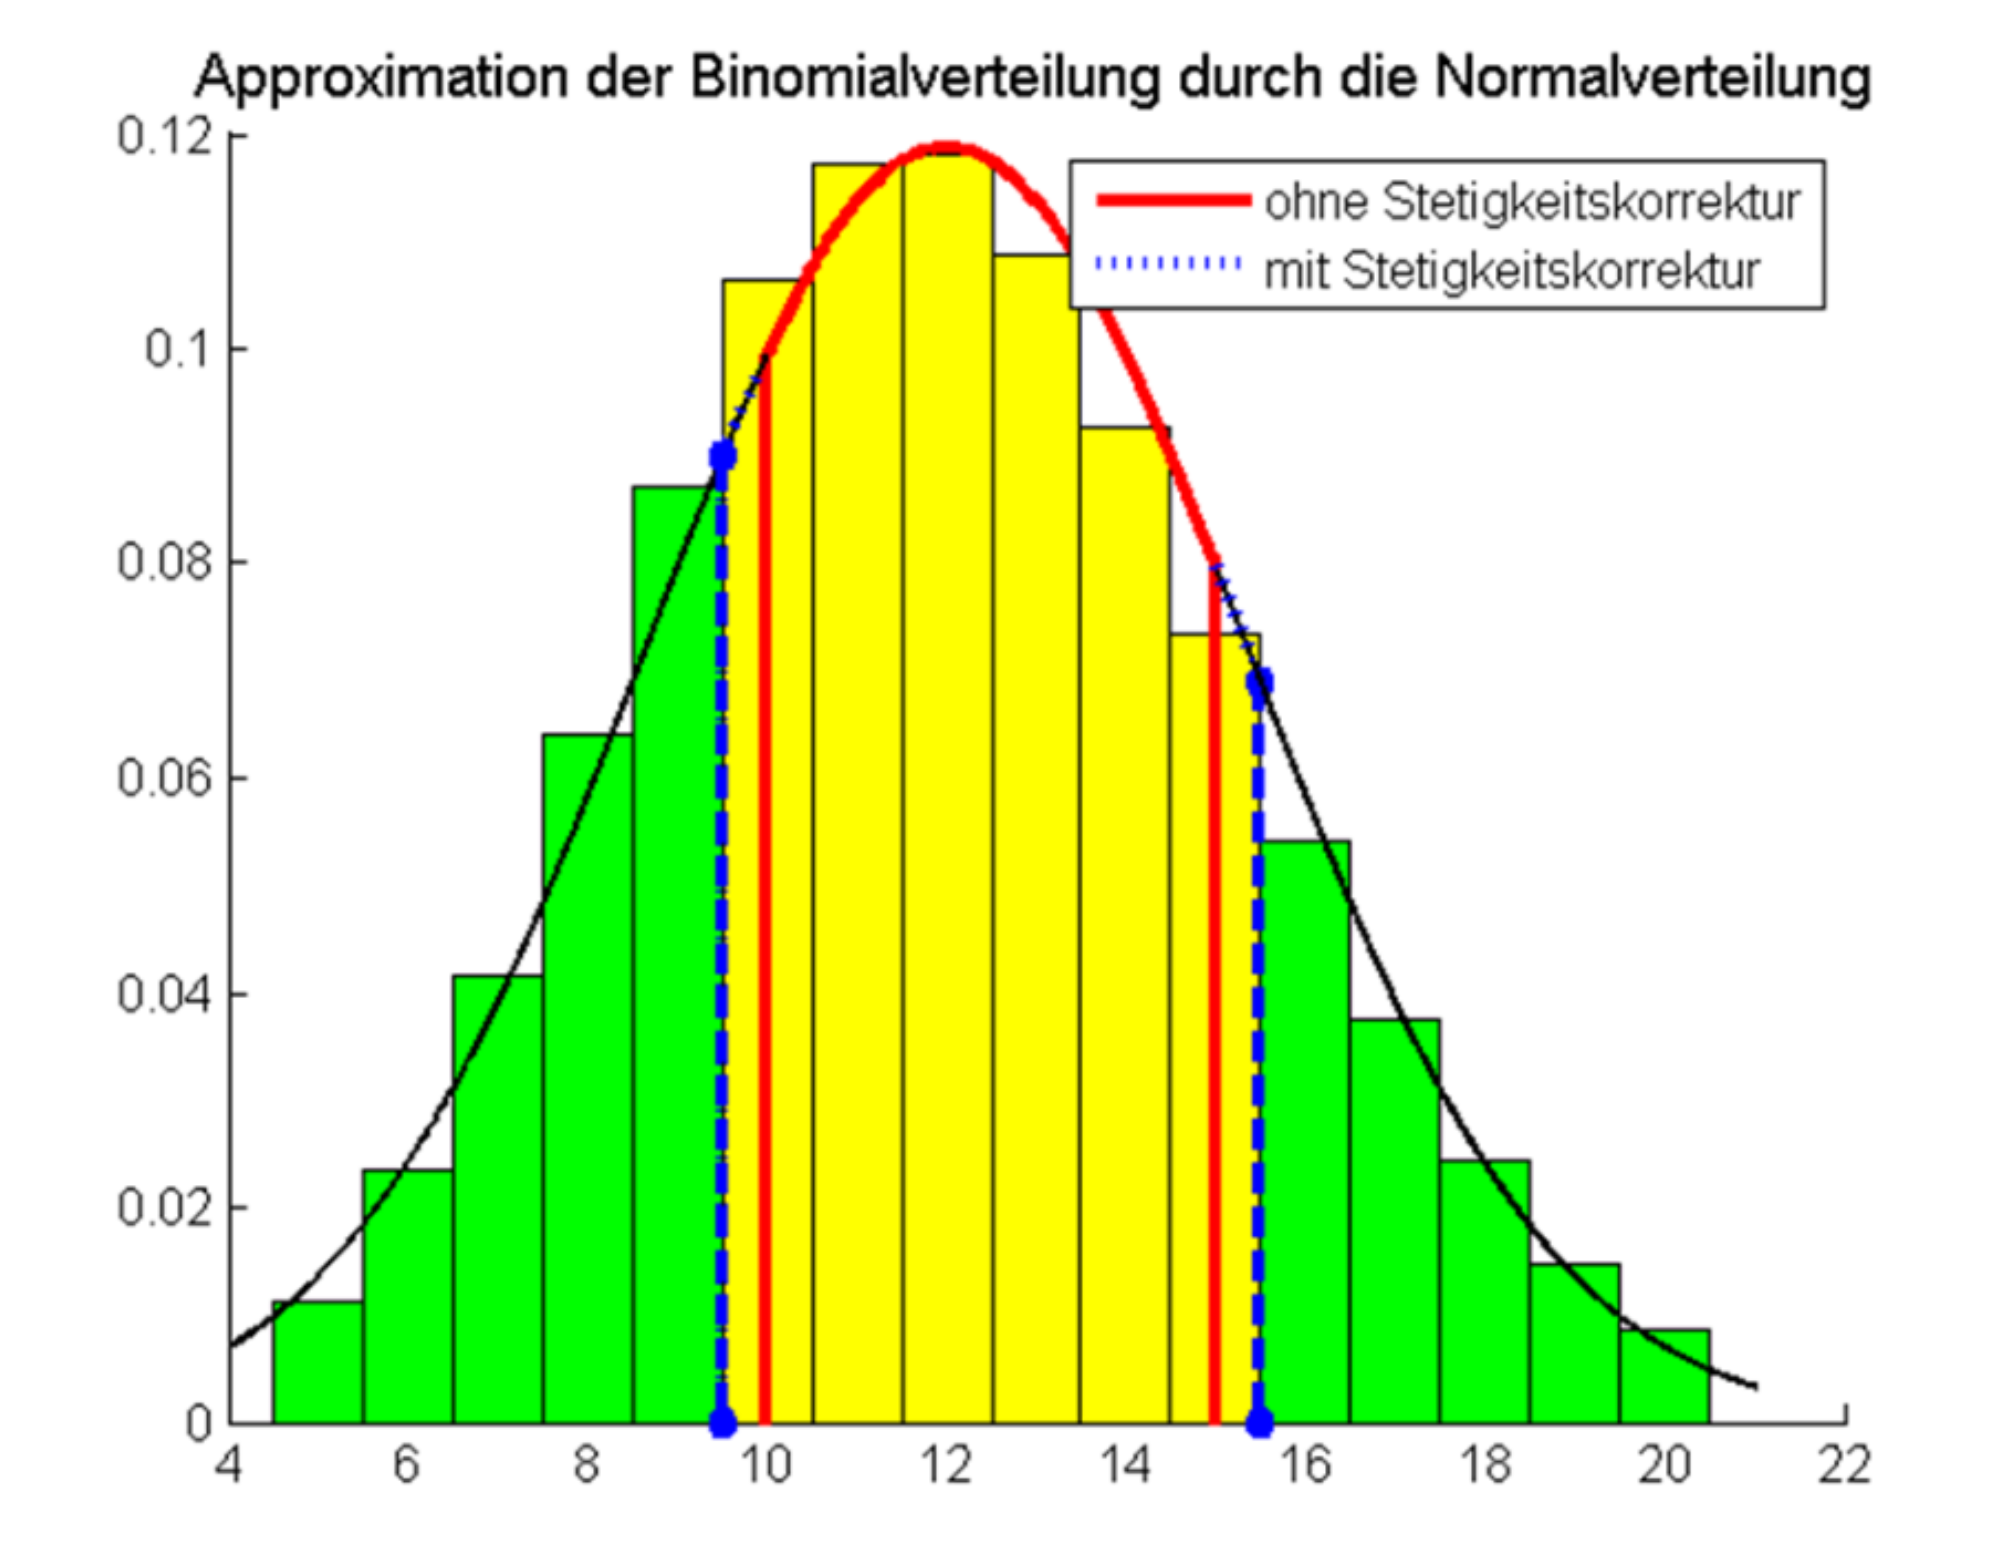
\includegraphics[width=\textwidth]{images/stetigkeitskorrektur.png}
                \begin{itemize}
                    \setlength\itemsep{0em}
                    \item $P(a \leq X \leq b) = \Phi_{\mu,\sigma}(b + \frac{1}{2})
                    - \Phi_{\mu,\sigma}(a - \frac{1}{2})$
                    \item $P(a < X \leq b) = \Phi_{\mu,\sigma}(b + \frac{1}{2})
                    - \Phi_{\mu,\sigma}(a + \frac{1}{2})$
                    \item $P(a < X < b) = \Phi_{\mu,\sigma}(b - \frac{1}{2})
                    - \Phi_{\mu,\sigma}(a + \frac{1}{2})$
                    \item $P(a \leq X < b) = \Phi_{\mu,\sigma}(b - \frac{1}{2})
                    - \Phi_{\mu,\sigma}(a - \frac{1}{2})$
                \end{itemize}
        \end{minipage}
    };
    \node[fancytitle, right=10pt] at (box.north west) {Stetigkeitskorrektur bei Approximationen};
    \end{tikzpicture}

\end{multicols}
\newpage







% --------------------------------------------------------------------
% Spezielle Verteilungen
% --------------------------------------------------------------------
\section*{Die Methode der kleinsten Quadrate}

\begin{multicols}{3}

% grundbegriffe
\begin{tikzpicture}
    \node [mybox] (box){
        \begin{minipage}{0.295\textwidth}
        \begin{tabular}{lp{6.5cm} l}
            $s_{xy}$: & Kovarianz\\
            $s_x^2$: & Varianz der $x_i$ Werte\\
            $s_y^2$: & Varianz der $y_i$ Werte\\
            $\hat{y}$: & Prognstizierte $y$-Werte\\
            $R$: & Bestimmtheitsmass\\
            $r_{xy}$: & Korrelationskoeffizient (S. 2)
        \end{tabular}
        \end{minipage}
    };
    \node[fancytitle, right=10pt] at (box.north west) {Grundbegriffe};
\end{tikzpicture}


\begin{tikzpicture}
    \node [mybox] (box){
        \begin{minipage}{0.295\textwidth}
            Die Regressionsgerade $g(x) = mx + d$ mit den Parametern $m$ und $d$
            ist die Gerade, für die die Residualvarianz $s_{\epsilon}^2$ minimal
            ist.
                \begin{itemize}
                    \setlength\itemsep{0em}
                    \item $m = \frac{s_{xy}}{s_x^2}$
                    \item $d = \overline{y} - m\overline{x}$
                    \item $s_{\epsilon}^2 = s_y^2 - \frac{s_{xy}^2}{s_x^2}$
                \end{itemize}
                \par\noindent\rule{\textwidth}{0.4pt}
                \begin{itemize}
                    \setlength\itemsep{0em}
                    \item $s_x^2 = \frac{1}{n}\sum\limits_{i=1}^{n} {(x_i - \overline{x})}^2 =
                    \left(\frac{1}{n}\sum\limits_{i=1}^{n} x_i^2 \right) - \overline{x}^2$
                    \item $s_y^2 = \frac{1}{n}\sum\limits_{i=1}^{n} {(y_i - \overline{y})}^2 =
                    \left(\frac{1}{n}\sum\limits_{i=1}^{n} y_i^2 \right) - \overline{y}^2$
                    \item $s_{xy} = \frac{1}{n}\sum\limits_{i=1}^{n} (x_i - \overline{x})(y_i - \overline{y})=\left(\frac{1}{n}\sum\limits_{i=1}^{n} x_iy_i \right) - \overline{x}\cdot\overline{y}$
                    \item $\overline{x} = \frac{1}{n}\sum\limits_{i=1}^{n}x_i$ und $\overline{y} = \frac{1}{n}\sum\limits_{i=1}^{n}y_i$
                \end{itemize}
        \end{minipage}
    };
    \node[fancytitle, right=10pt] at (box.north west) {Regressionsgerade};
    \end{tikzpicture}


\begin{tikzpicture}
    \node [mybox] (box){
        \begin{minipage}{0.295\textwidth}
            Die Totale Varianz setzt sich zusammen aus der Residualvarianz und
            der Varianz der prognostizierten Werte:\\
            \begin{itemize}
                \setlength\itemsep{0em}
                \item $s_{\hat{y}}^2 = m^2 s_x^2 = \frac{s_{xy}^2}{s_x^2}$
                \item $s_y^2 = s_{\epsilon}^2 + s_{\hat{y}}^2$
                \item $R^2 = \frac{s_{\hat{y}}^2}{s_y^2} = \frac{s_{xy}^2}{s_x^2 s_y^2} = r_{xy}^2$
            \end{itemize}
        \end{minipage}
    };
    \node[fancytitle, right=10pt] at (box.north west) {Bestimmtheitsmass};
    \end{tikzpicture}
\end{multicols}


% --------------------------------------------------------------------
% Spezielle Verteilungen
% --------------------------------------------------------------------
\section*{Schliessende Statistik}

\begin{multicols}{3}

\begin{tikzpicture}
    \node [mybox] (box){
        \begin{minipage}{0.295\textwidth}
        \begin{tabular}{lp{6.5cm} l}
            $\Theta_u$: & unteres Vertrauensintervall\\
            $\Theta_o$: & oberes Vertrauensintervall\\
            $\gamma$: & Sicherheit\\
        \end{tabular}
        \end{minipage}
    };
    \node[fancytitle, right=10pt] at (box.north west) {Grundbegriffe};
\end{tikzpicture}

\begin{tikzpicture}
    \node [mybox] (box){
        \begin{minipage}{0.4\textwidth}
            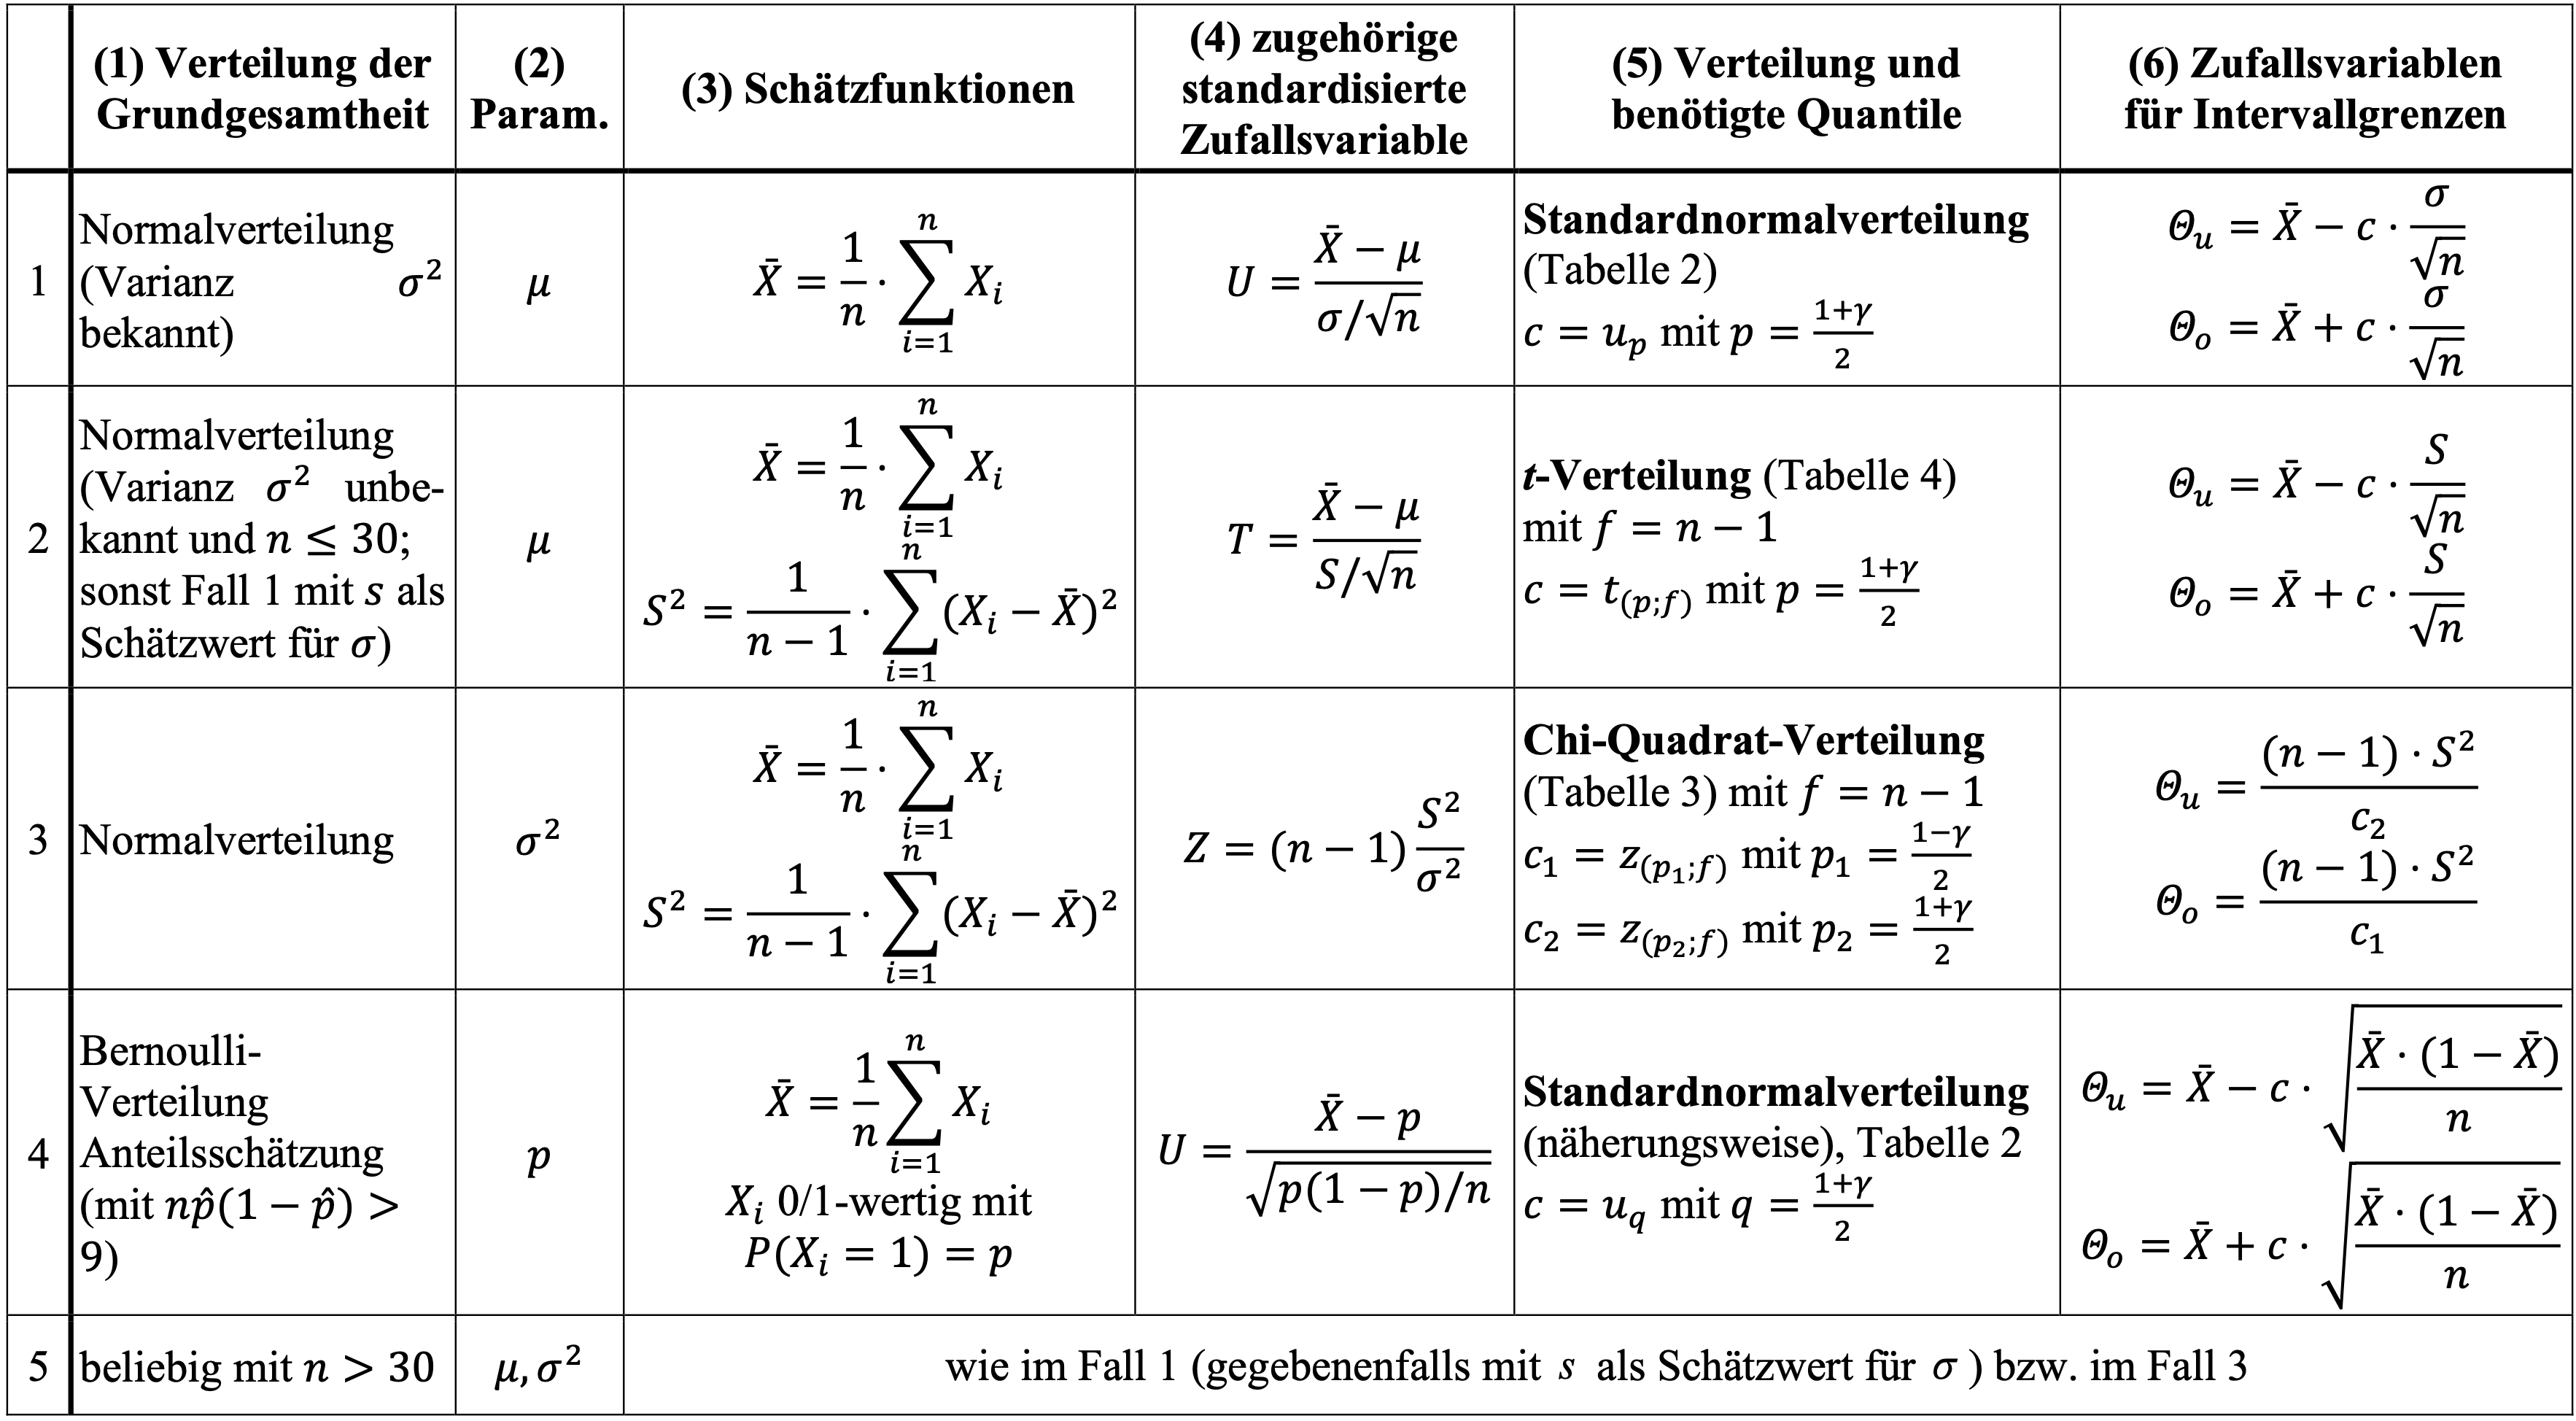
\includegraphics[width=\textwidth]{images/schliessende_sts.png}
        \end{minipage}
    };
    \node[fancytitle, right=10pt] at (box.north west) {übersicht Vertrauensintervalle};
    \end{tikzpicture}
\end{multicols}
\end{document}
